\documentclass[a4paper,twoside,twocolumn]{article}
\pdfoutput=1

\newif\iftr % \trtrue if for Tech Report
\trtrue     % \trfalse if not for Tech Report
%\newif\ifnony % \nonytrue if nonymised (ie nameful)
%\nonyfalse     % \nonyfalse if anonymised
\newif\ifccs   % \ccstrue if Concept Categorisation System visible
\ccstrue      % \ccsfalse if Concept Categorisation System invisible

% Test whether compiler is PDFLaTeX
\usepackage{ifpdf}  % Avoid \newif\ifpdf which clashes with same command
                    % in ifpdf package used by packages like hyperref
\ifpdf
    \usepackage[pdftex]{graphicx}
    \usepackage[colorlinks,linkcolor=blue,citecolor=blue,urlcolor=blue]{hyperref}
    \pdfcompresslevel=9 % Maximum compression
    \DeclareGraphicsExtensions{.pdf}
    % \usepackage[pdftex]{thumbpdf}      % thumbnails for pdflatex
    \pdfadjustspacing=1                % force LaTeX-like character spacing
\else
    \usepackage{graphicx}
    \usepackage[hypertex]{hyperref}  % supports hypertext in PDF but no Acrobat features e.g. bookmarks
\fi
% Common settings for hyperref are made in hyperref.cfg

% Load packages that require graphicx to have been loaded.
\usepackage{todonotes} % Allows insertion of \todo{} notes - uses graphicx package and clashes with pdftex option below
%\usepackage[disable]{todonotes} % Suppresses todo notes

% Load supported packages
\usepackage{
url       %
,fancyhdr % Fancy Headers
,lastpage % Creates marker with key LastPage, for pxxx of yyy to refer to.
,enumerate % More bullet styles
,amsmath  % AMS maths
,amsfonts % AMS fonts
,amssymb  % AMS symbols
%,moreverb % additional verbatim miscellany
%,amsthm   % AMS theorems defines proof environment
%,calc     % For calculations in length commands
%,newtheorems % Load after hyperref: see below
, enumitem % finer control of lists, e.g. \begin{itemize}[nosep] ... removes spacing
, array % for vertically centred cell contents in tabular and array environments
, xfrac % fraction extensions, such as slanted (\sfrac)
, multirow % multi-row tables
}
\newcolumntype{C}[1]{>{\centering\arraybackslash}p{#1}}
%\usepackage[force,almostfull]{textcomp} % Additional symbols, including generic currency
\usepackage[hang]{footmisc} % Hanging indent for footnotes
\setlength\footnotemargin{10pt}

% Load my personal packages
\usepackage[noindent, arraystretch, fullpage]{setlengths} % [noindent, arraystretch, {fullpage|tightpage|inchrndtext}]{setlengths}
\usepackage{
own         % Defines \newboolean{twocol}
}

% Load my personal packages
%\usepackage{
%newtheorems, % Defines theorem, definition, hypothesis, lemma \& assumption environments
%             % Note: \newtheorem must be used after \usepackage{hyperref} to ensure \theH<counter> is cross-referenced as well as \the<counter>
%}
%\usepackage{amsthm}
%\newtheorem{assumption}{Assumption}
%\newtheorem{requirement}{Requirement}
%\newtheorem*{test*}{Test}

\graphicspath{{images/}}

\newcommand{\pluseq}{\mathrel{+}=}

% Preamble metadata---------------------------------------------------
\newcommand*{\metaauthori}{Bob Briscoe}
\newcommand*{\metaauthorii}{}
\newcommand*{\metashorttitle}{Rapid Signalling of Queue Dynamics}
\newcommand*{\metatitle}{{\large{Technical Report}}\\Rapid Signalling of Queue Dynamics}
\newcommand*{\metano}{TR-BB-2017-001}
\newcommand*{\metakeywords}{Data Communication, Networks, Internet, Control, Congestion Control, Quality of Service, Performance, Latency, Responsiveness, Dynamics, Algorithm, Active Queue Management, AQM, Congestion Signalling, Sojourn time, Queue delay, Service time, Wait time, Expectation, Estimation, Blame, Fair marking, Burstiness, Cost-fairness, Explicit Congestion Notification, ECN, Packet Drop, Discard}
\newcommand*{\metahomepage}{\(<\)\href{http://bobbriscoe.net/}{http://bobbriscoe.net/}\(>\)}
\newcommand*{\metamaili}{\href{mailto:research@bobbriscoe.net}{research@bobbriscoe.net}}
\newcommand*{\metamailii}{}
\newcommand*{\metaaddress}{}
\newcommand*{\metatel}{Tel. +44 7718 902848}
\newcommand*{\metaversion}{04B}
\newcommand*{\metadate}{28 Nov 2021}

\hypersetup{                       % Set PDF document attributes
     pdfauthor = {\metaauthori%
     % and \metaauthorii
     },
     pdftitle = {\metashorttitle},
     pdfsubject = {},
     pdfkeywords = {\metakeywords}
}%

% Set document metadata
\title{\metatitle}%
\author{\metaauthori%
\thanks{\metamaili, %
\metaaddress}%
%\ %
%\and \metaauthorii%
%\thanks{\metamailii}%
}
\date{\metadate}%

% Running headers and footers
\pagestyle{fancy}%
\fancyhf{}%
\fancyhead[LO,RE]{\metashorttitle}%
\fancyhead[LE,RO]{\metano}%
\fancyfoot[LO,RE]{\scriptsize{\copyright~bobbriscoe.net Ltd, 2017-2018}}%
%\fancyfoot[LO,RE]{}%
\cfoot{\footnotesize{\scriptsize{Version~\metaversion}}}%
\fancyfoot[RO,LE]{\scriptsize{\thepage~of~\pageref{LastPage}}}%

\fancypagestyle{first}{%
\fancyhead[LO,RE]{}%
\fancyhead[LE,RO]{}%
%\fancyhead[C]{\Large Draft: Limited Review Distribution only}%
\fancyhead[C]{}%
\renewcommand{\headrulewidth}{0pt}%
}%

% Typesetting control
\pretolerance = 150%
%\tolerance = 250%
\tolerance = 5000%
\emergencystretch = 0 em%
% Typesetting overfull/underfull message control
%\hbadness = 150%
\hbadness = 4999%
\hfuzz = 0 pt%

% Set amsmath equation numbering to be relative to containing section
%\numberwithin{equation}{section}
\newcounter{ass}
\newcounter{req}

% Set Sectioning style
%\setcounter{secnumdepth}{3}
%\renewcommand{\baselinestretch}{1.2}
%\renewcommand{\bibname}{References}

% ----------------------------------------------------------------
\begin{document}
\bibliographystyle{alpha}%

% ----------------------------------------------------------------

\maketitle%
\thispagestyle{first}

% ----------------------------------------------------------------
\begin{abstract}
{\small\noindent%
% !TeX root = sigqdyn_tr.tex
% ================================================================
This paper focuses on reducing the delay before an active queue management (AQM) algorithm emits congestion signals, e.g.\ explicit congestion notification (ECN) or packet drop. These algorithmic delays can be greater than the delay that the data itself experiences within the queue. Once the congestion signals are delayed, regulation of the load becomes more sloppy, and the queue tends to overshoot and undershoot more as a result, leading the data itself to experience greater peaks in queuing delay as well as intermittent under-utilization. Also, even if an AQM algorithm only slightly delays its congestion signals, it tends to shift the signals from more bursty flows onto other smoother flows.

The importance of immediate congestion signalling has been recognized in approaches such as Data Center TCP (DCTCP) and Low Latency Low Loss Scalable throughput (L4S). However, this paper points out that the sojourn time metric that is increasingly used in these approaches introduces unnecessary internal measurement delay, which is worst during bursts. Expected service time is proposed as an alternative metric. Three potential implementations are proposed, which keep some or all of the benefits of sojourn time, but without the internal measurement delay. The paper also briefly surveys ways to remove other delays within AQMs, such as the delay due to randomness in the signal encoding.



}      % Abstract
\end{abstract}
%%% Categories, terms, and keywords %%%%%%%%%%%%%%%%%%%%%%%%%%%%%%%%%%%%%%%%%%%%
\ifccs{}%
%
% The code below should be generated by the tool at
% http://dl.acm.org/ccs.cfm
% Please copy and paste the code instead of the example below. 
%
\subsection*{CCS Concepts}
\textbf{\textbullet Networks} \(\to\) \textbf{Cross-layer protocols; Network algorithms; Network dynamics;}
% Print out keywords section
\subsubsection*{Keywords}
\metakeywords
%
\fi{}%

% !TeX root = sigqdyn_tr.tex
% ================================================================
\section{Introduction and Scope}\label{sigqdyntr_intro}

Much attention has been paid to reducing the delay experienced on the data path through packet networks. For instance, see sections II and IV of the extensive survey of latency reducing techniques in \cite{Briscoe14b:latency_survey}, which aim to reduce propagation delay, queuing delay, serialization delay, switching delay, medium acquisition delay and link error recovery delay.
%
%Propagation and queuing delay are typically the largest contributors to the overall delay experienced by network data.\footnote{For radio links medium acquisition delay is also highly significant.} Propagation delay can be reduced by structural techniques, such as server placement, but queuing delay is a result of subtle interactions due to the system design. 

This memo focuses on reducing unnecessary delays in the control system that attempts to match load to capacity. Reducing queuing delay has also been the focus of much other recent work. But the focus here is on cutting delays in the control path rather than the data path. That is, delays in measuring queue dynamics and in communicating the resulting control signals.

Once congestion signals are delayed, regulation of the load becomes more sloppy, and the queue tends to overshoot and undershoot more as a result, leading the data itself to experience greater peaks in queuing delay as well as intermittent under-utilization. And, perhaps most importantly, if the congestion signals due to bursts of data are delayed, even slightly, they will be applied to the packets just after each burst. Then bursty traffic could shift much of the blame for congestion onto other traffic running more smoothly in the background.

This memo applies to so-called immediate AQMs that intend to signal growth in the queue immediately. It is intended to ensure that packets carry signals that apply to those packets themselves, not to earlier packets, not even slightly earlier. Then signals intended to be applied to packet bursts will not be applied to packets after the burst. So-called Classic AQMs are not in scope because they deliberately filter out rapid variations in the queue before signalling more persistent queue growth, which introduces perhaps 100\,ms of smoothing delay.

To be concrete, this memo assumes congestion signals that are transmitted from an active queue management (AQM) algorithm~\cite{Adams13:AQM_survey} using either drop or explicit congestion notification (ECN)~\cite{Floyd94:ECN}, which are the only standardized signalling protocols~\cite{IETF_RFC3168:ECN_IP_TCP} for end-to-end use over one of the two Internet protocols, IPv4 and IPv6. The L4S ECN protocol~\cite{Briscoe15f:ecn-l4s-id_ID} is an experimental update to the standard ECN protocol intended to be used for immediate signalling of congestion. But the problems in this memo apply equally if an immediate AQM uses a different signalling protocol, such as the SCE~\cite{Morton19:SCE_ID} proposal. Most of the ideas concern only algorithmic improvements, which could be applied in other settings with completely different congestion signalling protocols.

\begin{figure*}
	\centering
	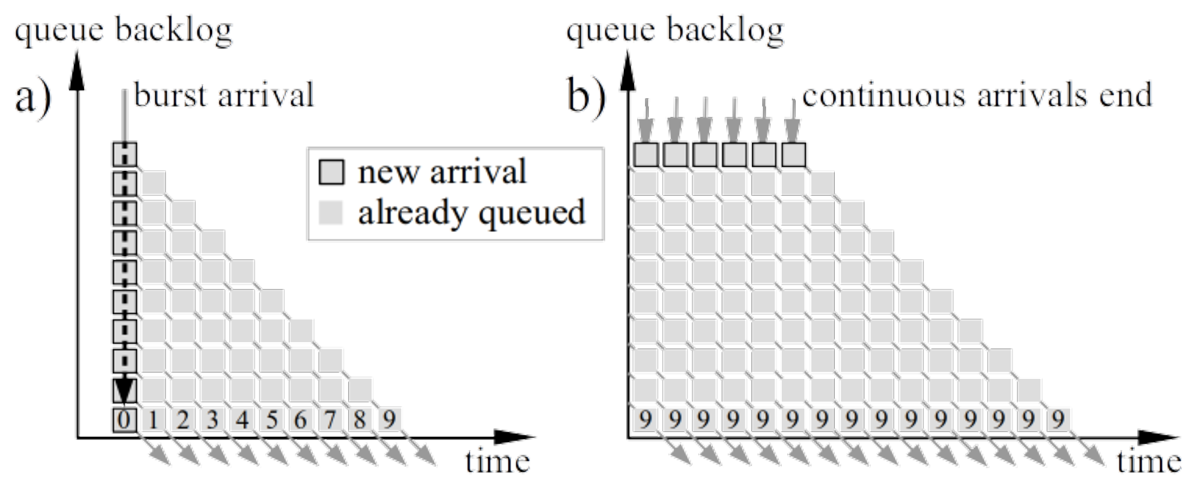
\includegraphics[width=0.8\linewidth]{sojourn-prob}
	\caption{Schematic Illustrating Two Problems with the Sojourn Time Metric. a) It does not measure the full size of a burst until the end (left); b) It does not measure a draining queue (right). Draining is visualized at one equisized packet per timeslot. Sojourn time is represented just before each packet is dequeued as the number of timeslots along its diagonal path.}\label{fig:sojourn-prob}
\end{figure*}

Control path delay consists of the following elements:
\begin{itemize}[nosep]
	\item propagation delay (in common with the data);
	\item queuing delay (in common with the data);
	\item measurement delay: measuring the queue, as well as arrival and/or departure rates;
	\item smoothing delay: filtering out fluctuations in measurements;
	\item signal encoding delay: a number representing the signal is produced within an AQM algorithm, which is then compressed into a unary `encoding' in each packet, and `decoded' by the congestion control algorithm's response to the unary-encoded signals. A unary encoding is used so that the AQM does not have to recognize flows or hold per-flow state. But it constrains the bandwidth of the signalling channel, which introduces encoding delay;
	\item randomization delay: randomness is introduced to break up oscillations, but it requires longer to detect the underlying signal.
\end{itemize}

This memo pays most attention to two of these: measurement and queuing delay. The other four are briefly surveyed in \S\,\ref{sec:related}.
      % Intro
% !TeX root = sigqdyn_tr.tex
% ----------------------------------------------------------------
\subsection{The Time to Measure the Service Time of a Queue}\label{sec:svc_time}

In around 2012, it became recognized that one of the main problems with AQMs was the sensitivy of their configuration to changing environments. For example:
\begin{itemize}
	\item access links often change their rate when modems retrain in response to interference. 
	\item a queue can be part of a scheduling hierarchy and traffic in higher priority queues varies the capacity left for a lower priority queue, rapidly varying the drain rate that the AQM experiences.
	\item the rate of typical WiFi links varies rapidly over time~\cite{McGregor10:Minstrel_TR}.
\end{itemize}

The CoDel algorithm~\cite{Nichols12:CoDel} proposed to solve this problem by measuring the queue in units of time, rather than bytes. This made the configuration of the thresholds in the algorithm independent of the drain rate.

Actually, as far back as 2002, 
Kwon and Fahmy~\cite{Kwon02:Load_v_Queue_AQM} had advised that the queue should 
be measured in units of time. Also, in 2003, S{\aa}gfors \emph{et al} had 
modified the Packet Discard Prevention Counter (PDPC+~\cite{Sagfors03:PDPC_vary}) 
algorithm by converting queue length to queuing delay to cope with the varying 
link rate of 3G wireless networks. PDCP still measured the queue in bytes, but then converted the result to time by dividing by the link rate, which it measured over a brief interval. 

CoDel proposed an elegant way to measure the service time of the queue by adding a timestamp to each packet's internal metadata on enqueue. Then at dequeue, it subtracted this timestamp from the system time. The authors called the result the sojourn time of the packet. It was also pointed out that this sojourn time could be measured over an arbitrarily complex structure of queues, even across distributed input and output processors.

Because PIE~\cite{Pan13:PIE} was initially designed for implementation using existing hardware, it did not measure the service time of the queue directly using the time-stamping approach of CoDel.
Instead, like PDPC, it converted queue length to queuing delay using a regularly updated 
estimate of the link rate, measured over a set amount of packets. When there were insufficient packets in the queue to measure the link rate or the rate was varying rapidly, PIE's estimate of the link rate became stale. So in later specifications of PIE~\cite{Pan17:PIE}, it recommended the sojourn approach of CoDel that had originally been designed for software implementation.

The queue length (in bytes or an equivalent unit), also called the backlog, can be measured instantaneously when a packet is enqueued or when it is dequeued. In contrast, it takes a sojourn time to measure sojourn time (which can only be measured as a packet is dequeued). So measuring sojourn time inherently introduces delay into the control path.

To minimize delay, the signal should be applied at dequeue. However, in some hardware pipelines the process of preparing link layer frames, including potential encryption, compression and framing, is already in progress by the time a packet is dequeued. So it is too late to mark or drop a packet. This is one reason that PIE initially applied the congestion signal when it enqueued a packet. That is, it probabilistically dropped (or ECN-marked) the packet when it enqueued it. This signal then worked its way through the queue before being transmitted, adding a sojourn time of delay to the signal. This is still the case for DOCSIS PIE, but software variants of PIE now apply marking or dropping at dequeue. 

The matrix in \autoref{tab:added-delay} shows the delay added to the signal by various techniques for measuring queue delay that will be introduced later (horizontal) and the two choices for where to apply the signal (vertical). It uses the following terminology: \(t_r\) is the duration used to sample the drain rate and \(t_s\) is the sojourn time. 
\begin{table}[h]
\begin{center}
\begin{tabular}{p{0.17\columnwidth}|C{0.16\columnwidth}*{2}{C{0.2\columnwidth}}}
\multirow{3}{0.17\columnwidth}
{Where signal is applied}
			& \multicolumn{3}{c}{Technique to measure queue delay}\\
			& \multirow{2}{0.17\columnwidth}
			  {Sojourn Time}
			            & \multicolumn{2}{C{0.5\columnwidth}}
			              {Expected Service Time}\\
                          \cline{3-4}
			&			& Time-Based Backlog&  Scaled Sojourn Time\\\hline 
	at enq  & \(2t_s\)	& \(t_r + t_s\)	& \(3t_s/2\)\\
	at deq  & \(t_s\)	& \(t_r\)			& \(t_s/2\)
\end{tabular}
\caption{Delay added to congestion signal by three different measurement techniques}%
\label{tab:added-delay}
\end{center}
\end{table}

The centre column shows the effective delay added by the simple `Time-Based Backlog' technique proposed in \S\,\ref{sec:time-based_backlog}. It also applies to the variant of that technique called `Size-Adjusted Threshold' in \S\,\ref{sec:time-adj_thresh}. The right hand column shows the delay of a technique called `Scaled Sojourn Time' introduced in \S\,\ref{sec:scaled_svc_time}, which can be used where the ability of sojourn time to measure delay across a complex set of queues is required. Nonetheless, for a simple software queue, the time-based backlog is preferable, because it always adds minimal measurement delay.

It can be clearly seen that applying a signal at enqueue adds \(t_s\) to the signal delay.
So applying the signal at enqueue would only be appropriate if it were not possible to mark (or drop) a packet at the head of the queue, e.g.\ due to implementation or timing constraints.

% ----------------------------------------------------------------
\subsection{The Blame Shifting Problem}\label{sec:fairer_marking}

When the Random Early Detection (RED) AQM algorithm was first proposed, fairness was one evaluation factor~\cite[\S\,8]{Floyd93:RED}. Fairness in the context of marking was defined as ``the fraction of marked packets for each connection is roughly proportional to that connection’s share of the bandwidth''. 

Such fairness would be sufficient if all flows were long lived and smooth, but they are not.  Wischik~\cite{Wischik99:Mark_Fairly} contrives a simple two-flow scenario to demonstrate how RED can shift nearly all the marking from a burst in one flow onto a smoother flow that continues after the burst. %In this scenario one flow usually sends at a lower rate than the other, but then suddenly causes congestion by sending faster for a brief period before returning to its lower rate. The queue smoothing algorithm within the RED AQM delays nearly all the congestion marking until after the congested period ends, when most arrivals are from the constant flow. 

Classical AQMs like RED or more recent designs such as CoDel or PIE are designed to filter out variations in the queue over a likely maximum round trip. So they inherently introduce smoothing delay of about 100--200\,ms prior to signalling congestion, which is far too long to be able to mark packet bursts correctly. More recently, the importance of immediate congestion signalling has been recognized in approaches such as Data Center TCP (DCTCP~\cite{Alizadeh10:DCTCP}) and Low Latency Low Loss Scalable throughput (L4S~\cite{Briscoe16a:l4s-arch_ID}), where the job of smoothing out variations is shifted from the AQM to the sender.

Marking fairness has been termed `shadow pricing'~\cite{Kelly98:Shadow_prices_prop_fair} or `cost fairness'~\cite{Briscoe06g:Rate_fair_Dis}, because it ensures the cost or harm to others of each user's behaviour can be measured. Note that marking fairness is an important mechanism requirement for all AQMs and should not be confused with flow-rate `fairness', which is an arbitrary policy choice concerning allocation of benefits at any instant (which is why `fairness' is placed in quotes in this latter case)\footnote{The RED paper went on to explain that ``RED gateways do not attempt to ensure that each connection receives the same fraction of the total throughput''.}. 

This section introduces fairness problems when sojourn time is used to mark flows with different degrees of burstiness. Then it uses a worked example to give better intuition for how to make marking fairer. The question of what marking would actually be fair for different degrees of burstiness is deferred to a later discussion section (\S\,\ref{sec:marking_fairness_discuss}). 

Nonetheless, we will now demonstrate that even the delay spent measuring sojourn time is enough to cause immediate marking to miss packet bursts, and hit smoother flows instead. Although we cannot yet say exactly what is fair, we can recognize this shift of blame, when one marking approach is significantly less fair than another.

\begin{figure}[h]
	\centering
	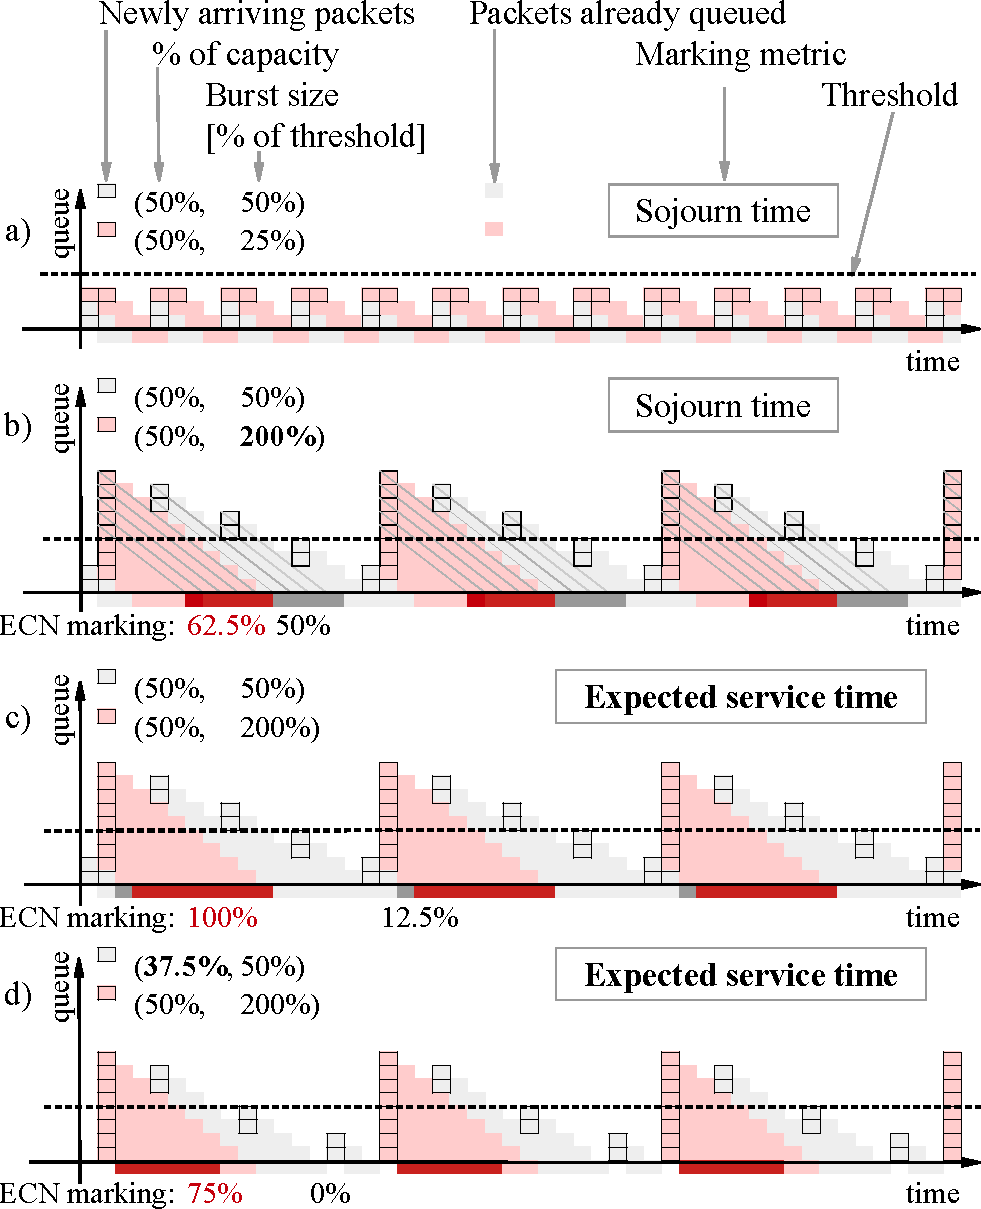
\includegraphics[width=\columnwidth]{marking-fairness5050}
	\caption{The Blame Shifting Problem and a way to solve it by replacing Sojourn Time with an Expected Service Time (EST) metric. %A time-series of the queue in a progression of simplified scenarios (a--d) is shown, with one change at a time, each highlighted in bold. a) is the baseline with grey:pink average arrival ratio of 50:50 and both with low burstiness. In both b) \& c) the two flows rates continue to average 50:50 but the pink flow arrives in larger, less frequent bursts. In c) the traffic is the same as b), but the marking algorithm is different; the dark red and dark grey packets below each x-axis indicate congestion-marked packets. Scenario d) illustrates the grey flow starting to respond to the congestion marking, while the pink flow remains unresponsive
	ECN marking (shown as darker packets under each x-axis) ought to indicate which packets are most to blame for queuing. But in (b) uing a sojourn metric, the pink bursts cause grey packets to attract nearly as much marking as pink. In (c) \& (d), the expected service time metric better ensures that ECN marking reflects the blame for any queuing. See text for full explanation and commentary.}\label{fig:marking-fairness5050}
\end{figure}

\autoref{fig:marking-fairness5050} shows how a packet queue behaves in a progression of four scenarios reduced to their essentials by using equal-sized packets; one timeslot per delivered packet; a constant rate link; a step ECN marking threshold (the dashed horizontal line); and high link utilization; but without modelling the interaction with the sender's congestion control. 

In the first three scenarios (a--c), two flows (grey and pink) fully utilize the link, consuming 50\% each. Newly arriving packets have a border while packets already queued do not, as shown in the legend above the top scenario. In all four scenarios, the grey packets arrive in small bursts, each the size of half the queue delay threshold. Other aspects of the traffic and marking algorithm change over the progression of scenarios, as highlighted in bold in each row of the figure and described below:
\begin{enumerate}[nosep, label=\alph*)]
	\item This is the baseline case to show that the pink flow can fill the capacity left by the grey flow without exceeding the threshold, as long as it keeps its bursts small enough (in this case just 25\% of the threshold, making at most 75\% if a pink burst were to coincide with a grey one). 
	\item In this case, each burst from the pink flow occupies 200\% not 25\% of the threshold in the buffer. The average rate of both flows is unchanged, so the link is still 100\% utilized, and the grey flow still arrives in the same pattern of small bursts. So, in the time the pink burst takes to drain, some of the smaller grey bursts back up behind it and, while they are draining, more small grey bursts accumulate. So the queue only finally empties just as the cycle starts to repeat with the arrival of the next pink burst.
	\item The arrivals in this scenario are identical to (b), but sojourn-based queue measurement is replaced with expected service time (EST---described below).
	\item In this last case, we attempt to represent the grey flow starting to respond to the ECN marking in (c), while the pink flow remains unresponsive at 50\% of the link and still arriving in large bursts twice the depth of the threshold. The flow rate of the grey flow reduces from 50\% to 37.5\% of the link or \(\sfrac{3}{4}\) of the rate of the pink flow.
\end{enumerate}

The ECN marking metric is written in the box above each scenario:
\begin{description}
	\item[Sojourn time:] In scenario b) in \autoref{fig:marking-fairness5050}, each diagonal darker line traces the sojourn through the queue of those packets that arrive when the queue is above the threshold. The service time or sojourn time of these packets will have exceeded the threshold so they will be marked on departure (shown under the axis as darker coloured packets). The proportion of marked packets of each colour is written under that.

	\item[Expected Service Time:] In scenarios c) or d) there are no diagonal lines, because, rather than measuring the delay of the packet itself, EST measures the delay that a packet causes to others. Various ways in which EST has been or could be implemented will be given in \S\,\ref{sec:exp_svc_time}, but briefly, instead of marking a packet based on the queue in front of it, EST estimates the queue delay \textit{behind} a packet at the instant it departs. In the schematic, EST marks departing packets (darker coloured) if the vertical depth of the queue in the timeslot just before departure exceeds the threshold.\footnote{The EST algorithm uses queue delay, but in this simplified illustration queue depth represents delay because the drain rate is constant.}
\end{description}

In this second pass, we comment on the ECN marking outcome from each scenario:
\begin{enumerate}[nosep, label=\alph*)]
	\item There is no ECN marking in this baseline case (whatever the metric).
	\item The sojourn times of 5/8 of the packets at the tail of the pink burst exceed the threshold. So the sojourn-based AQM marks 62.5\% of the pink packets at dequeue. Because grey packets back up, first behind the pink burst then behind themselves, their sojourn times exceed the threshold for the first 50\% of the grey packets between each pair of pink bursts. Thus, the marking probability of the pink flow is only slightly greater than the grey, even though the pink flow's excessive burstiness is largely to blame for the queue exceeding the threshold.\footnote{Indeed, if each pink burst had happened to arrive one timeslot later, its marking would have been the same as the grey.}
	\item Here the evolution of the queue is identical to scenario (b), but marking is based on the `Expected service time' (EST) metric described above. This increases the pink marking probability from 62.5\% to 100\%, because every pink packet in the burst has caused a queue to back up behind it. In contrast, EST only marks one grey packet in each pink burst cycle --- the one that the pink burst happens to arrive behind. Thus grey marking reduces to 12.5\%, compared to 50\% with the sojourn metric.
	\item As the load from responsive grey traffic falls a little, after each unresponsive pink burst the queue falls below the threshold considerably sooner. This completely removes all grey marking, thus rewarding the grey flow for its responsiveness without too much under-utilization. The grey flow's response also reduces pink marking, but only to 75\%.
\end{enumerate}

The wider space of scenarios like this has been investigated by varying the relative shares and relative burst sizes between flows (see \S\,\ref{sec:marking_fairness_discuss}). Although the difference between the sojourn and expected service time metrics is sometimes less dramatic and sometimes more, the following intuition is generally true for all scenarios.

A smoother flow has smaller but more frequent arrival events compared to a bursty flow. So, although the bursty flow might happen to back up behind one of the smaller bursts of the smoother flow, multiple arrival events of the smoother flow will back up behind the larger burst. Therefore proportionately more of a bursty flow will be near the head of the buffer, and the packets of a smoother flow will be more likely to be occupying the tail. Figures \ref{fig:marking-fairness8020} \& \ref{fig:marking-fairness8020_4} illustrate this general point with a couple of different example traffic models.

\begin{figure}[h]
	\centering
	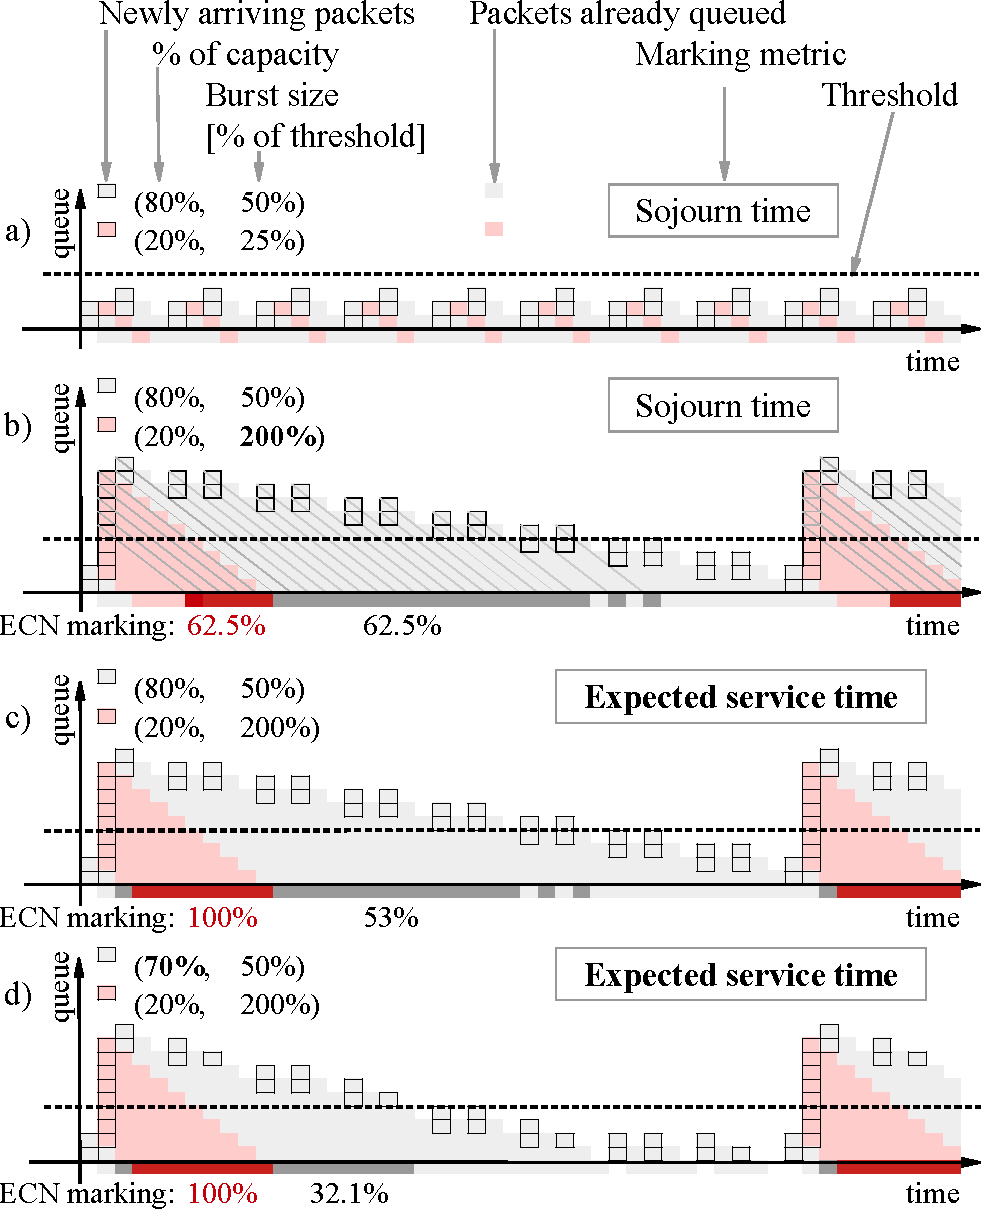
\includegraphics[width=\columnwidth]{marking-fairness8020}
	\caption{The Blame Shifting Problem with a minority of bursty unresponsive traffic using the sojourn metric (pink), and a solution using an EST metric.}\label{fig:marking-fairness8020}
\end{figure}

The grey:pink ratio in \autoref{fig:marking-fairness8020} is 80:20 rather than 50:50, but other aspects like burst sizes are the same as in \autoref{fig:marking-fairness5050}. \autoref{fig:marking-fairness8020}b) shows that the sojourn metric still allows the pink bursts to shift about half the blame for marking onto the grey flow. In contrast, EST marking (\autoref{fig:marking-fairness8020}c) again subjects the pink flow to the maximum possible blame (100\% marking). But this time the grey flow still attracts a little over 50\% marking, which reflects the greater proportion of the link that it consumes. 

Nonetheless, a slight grey reduction to \(\sfrac{7}{8}\) of its previous rate (\autoref{fig:marking-fairness8020}d), reduces its marking to just over 30\%, while still subjecting the bursty pink flow to 100\% marking. With sojourn marking, the same reduction by the grey flow would have reduced its marking to 37.5\% (not shown). So by shifting less blame to the grey flow, EST will lead to less underutilization than sojourn in steady state. EST also continues to attribute a higher degree of blame to the unresponsive pink bursts (100\% marking). Also, a congestion policer driven by EST marking would discriminate between the flows better than if driven by sojourn.

\begin{figure}[h]
	\centering
	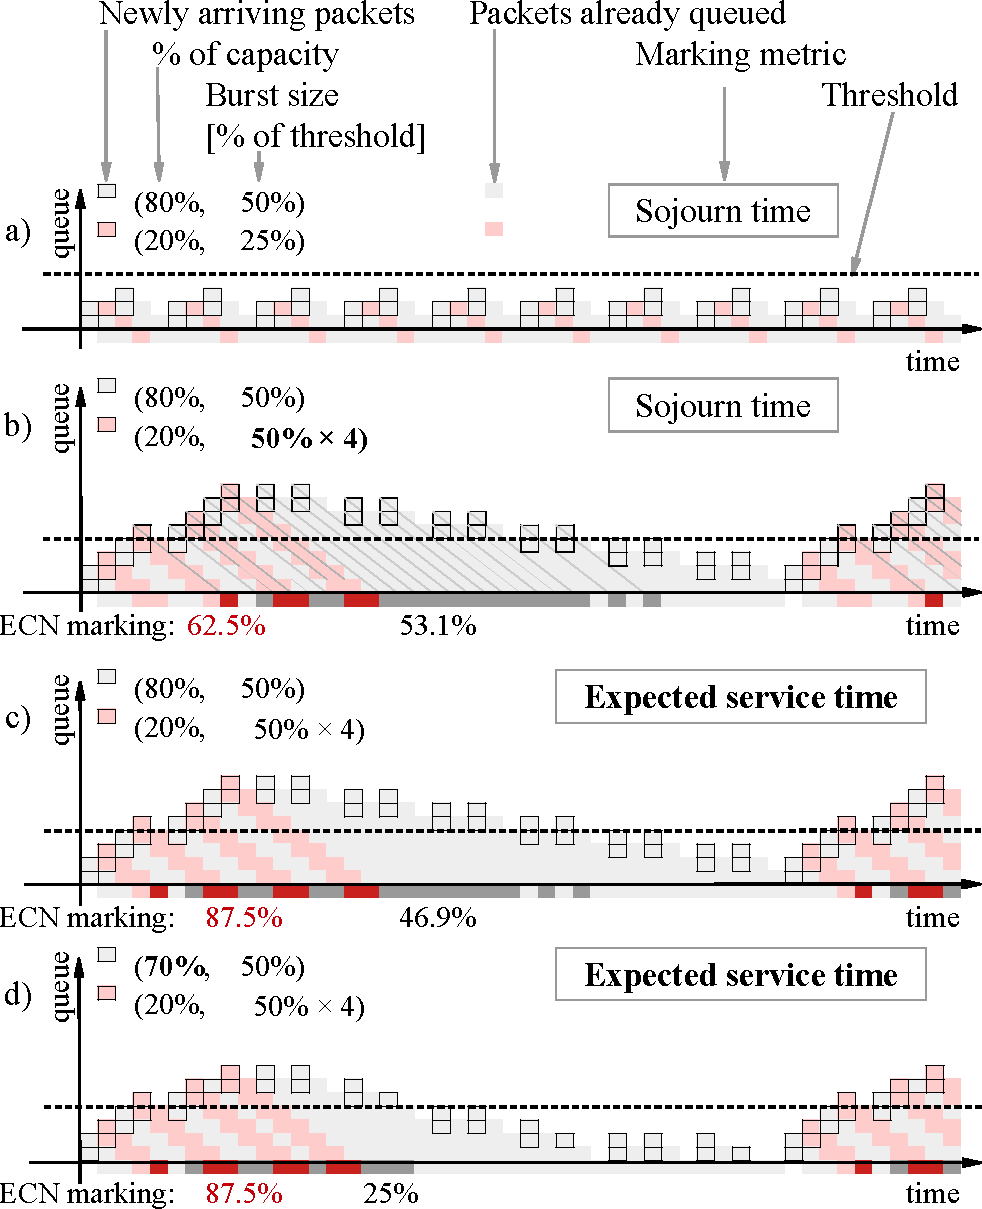
\includegraphics[width=\columnwidth]{marking-fairness8020_4}
	\caption{The Blame Shifting Problem with the sojourn metric using two flows of equal burstiness; one continuous (grey); the other intermittent (pink). And a solution using an EST metric.}\label{fig:marking-fairness8020_4}
\end{figure}

The traffic model in \autoref{fig:marking-fairness8020_4} is similar to the grey:pink 80:20 case in \autoref{fig:marking-fairness8020} except the pink flow divides the one burst into four smaller bursts of the same size (50\% of the threshold) and paced at the same rate as the continual grey bursts. Sojourn-based marking results in the same 62.5\% pink marking probability as in Figures \ref{fig:marking-fairness5050} \& \ref{fig:marking-fairness5050}. But grey marking is slightly lower than either. This is because sojourn-based marking reflects `harm to self due to others packets' and there is less pink burstiness. In contrast, with EST (\autoref{fig:marking-fairness8020_4}c), pink marking is higher and grey is lower, but the improvement is not as pronounced as in \autoref{fig:marking-fairness8020}c). In \autoref{fig:marking-fairness8020}d), the grey traffic reduces its own marking considerably by reduces its average pacing rate a little, but without affording any benefit to the unresponsive pink traffic. 

It may seem wrong that EST marks pink traffic more than grey, when pink paces at the same rate as grey but for less of the time. However, it is only the proportion of pink marking that is greater. In \autoref{fig:marking-fairness8020_4}c) there are four times as many grey packets as pink. So, even though pink marking approaches double the proportion of grey, the absolute number of pink markings is less then half that of grey. While the pink flow is active, the sum of pink and grey exceeds the link capacity, so EST `punishes' both equally. But then EST stops marking the rest of the grey traffic as a reward for allowing the queue to recover by underutilizing the link.

So far, on the limited evidence of a few simple cases, we can draw the interim conclusion that marking the head packet when there is an excessive backlog behind it is likely to lead to fairer marking than marking the head packet because it experienced a backlog in front of it that held up its own sojourn through the queue. 

% ----------------------------------------------------------------
\subsection{Implications of Unfair Marking}\label{sec:effects_unfair_marking}

\paragraph{Blame shifting with bursty traffic:} The section ``Underutilization with Bursty Traffic'' of Heist and Morton's write-up \cite{Heist20:L4S_tests} injects large bursts of unresponsive traffic into a queue that applies immediate ECN marking above a shallow threshold based on the sojourn metric. When there is also smoothly paced traffic in the same queue, the bursts cause the AQM to focus more ECN markings onto the smooth traffic, and less on the bursts. Thus, using the sojourn metric allows bursty traffic to shift the blame for the queuing it causes onto smooth traffic.

This effect can be exploited to cause smoother traffic to yield more to bursty traffic. If the bursty traffic is also unresponsive itself (as it was in \cite{Heist20:L4S_tests}), it causes the smooth traffic to significantly underutilize the link. Thus, it is important to ensure that ECN marking reflects the blame for any queuing (\S\,\ref{sec:marking_fairness_definition} discusses how to quantify the apportionment of blame objectively).

The section ``Underutilization with Bursty Links'' in the same online collection of tests~\cite{Heist20:L4S_tests} shows a similar effect. When the traffic transmitted by a smooth link (e.g.\ fixed Ethernet) is mixed with traffic that has traversed a bursty link (e.g.\ WiFi), the bursty traffic causes a sojourn-based immediate AQM to shift its marking onto the smooth traffic.

\paragraph{Perverting congestion policing:} A common technique in traffic policing is to identify misbehaving traffic by the disproportionate amount of congestion marking that an AQM applies to it, as first proposed by Floyd and Fall~\cite{Floyd99:Penalty_box}. Therefore, if an AQM fails to subject bursty traffic to a fair degree of marking, it will allow bursty traffic both to evade policing and to fool the policer into punishing smoother traffic instead.\footnote{See \S\,\ref{sec:qprot_marking_fairness} for a potential efficiency improvement to queue protection based on EST marking.}

\paragraph{Late-comer Disadvantage:} TCP Segmentation Offload (TSO) in Linux (and possibly other OSs) groups a set of packet into a back-to-back aggregate or burst and calculates the maximum packets in a burst from the current pacing rate of the flow (in pkt/s):
\[\mathrm{max\_burst} = \mathrm{pacing\_rate}\times \frac{\mathrm{MAX\_BURST\_DELAY}}{\mathrm{MTU\_BITS}}.\]
The flow's pacing rate is upper bounded by the link rate, so this ensures that the burst will not cause more than MAX\_BURST\_DELAY of queuing delay at the bottleneck. However, when a new flow starts, its pacing rate is typically well below the link rate and well below the pacing rate of any flows already established over the bottleneck link. Therefore new Linux flows consist of smaller bursts while established Linux flows consist of larger bursts. 

If an AQM at the bottleneck is based on sojourn time and therefore marks larger bursts less than smaller bursts, new flows will attract a higher congestion marking probability than established flows. Then as a new flow tries to displace an established flow, it will tend to reach a point of local equilibrium before it has reached the same rate as the established flow. Thus sojourn marking can lead to a late-comer disadvantage.

\bob{Add figures from Joakim's paper}.

% ----------------------------------------------------------------
\subsection{Blame Shifting and Per-Flow Queueing}\label{sec:fq_blame_shifting}

\begin{figure}[h]
	\centering
	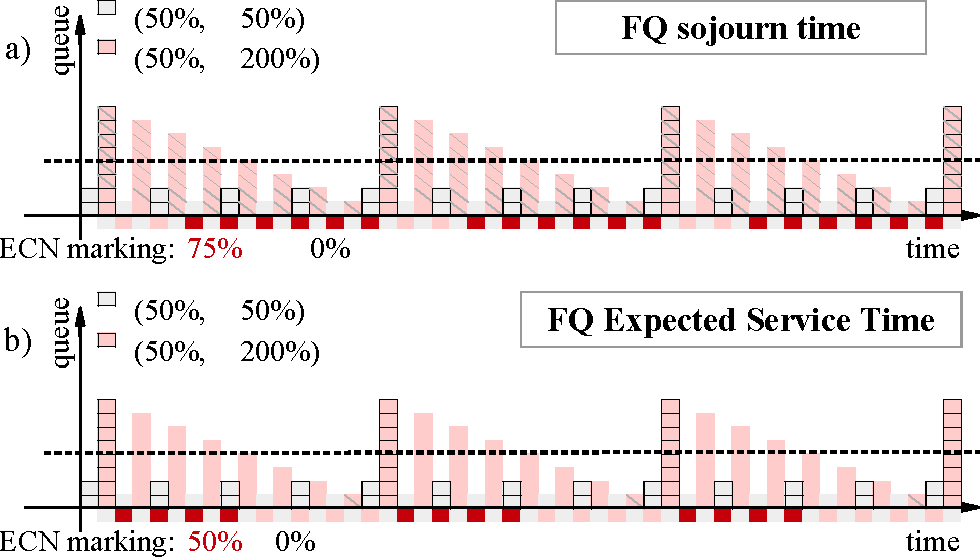
\includegraphics[width=\columnwidth]{fq-marking-fairness5050}
	\caption{Per-flow queuing (FQ) provides isolation for the grey flow from the pink bursts in the simple case of 50:50 capacity shares. Each timeslot shows only the flow-queue being served in that slot. Note that the visualization of the marking threshold is no longer useful, because the height of each queue no longer represents its delay when more than one queue is being served.}\label{fig:fq-marking-fairness5050}
\end{figure}

Heist and Morton \cite{Heist20:L4S_tests} suggest that per-flow queuing (FQ) would probably provide isolation for smooth flows from bursts. This could be true in some cases, such as the case with a more bursty pink flow sharing capacity 50:50 with a smoother flow, as shown in \autoref{fig:fq-marking-fairness5050}. Here, irrespective of whether marking is sojourn or EST-based, 75\% is focused on the pink bursts, and none on the grey flow.

\begin{figure}[h]
	\centering
	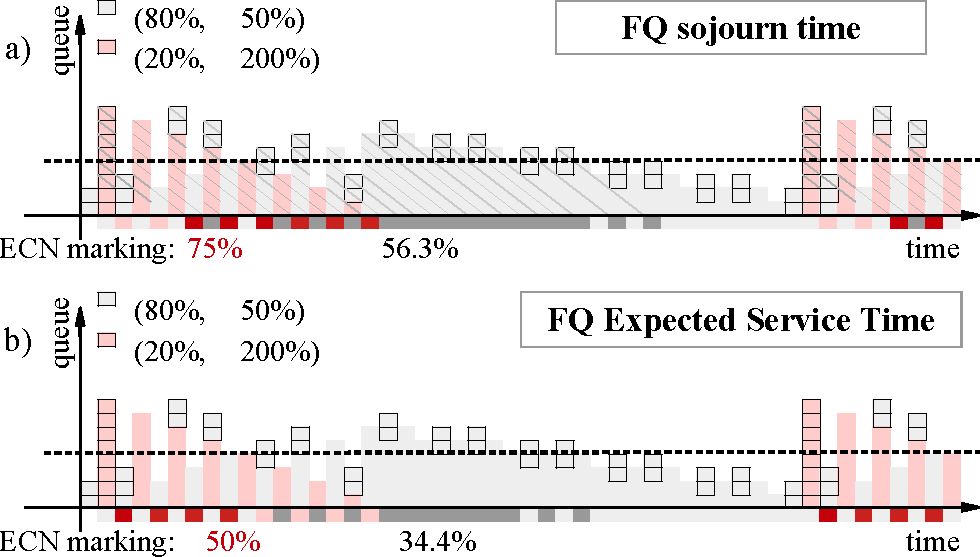
\includegraphics[width=\columnwidth]{fq-marking-fairness8020}
	\caption{FQ does not isolate the smooth grey flow from the pink bursts when their capacity shares are 80:20. FQ paces the burst better than a FIFO, but it still makes the grey flow queue up behind the burst, which it would not have done if the pink flow had arrived evenly paced. EST-based marking (b) shifts somewhat less blame onto the smooth grey flow than sojourn (a).}\label{fig:fq-marking-fairness8020}
\end{figure}

However, Figures \ref{fig:fq-marking-fairness8020} \& \ref{fig:fq-marking-fairness8020_4} show that isolation between flows breaks down for the 80:20 traffic models introduced earlier in Figures \ref{fig:marking-fairness8020} \& \ref{fig:marking-fairness8020_4}. Note here that, when grey packets arrive in a timeslot when pink packets are being served, they are shown queuing behind the pink queue (to show the slot when their sojourn timer starts), but they are then shifted into the correct queue in the next slot.

\autoref{fig:fq-marking-fairness8020}a) illustrates that this is because the scheduler serves the grey flow more slowly until it has delivered the whole of the pink burst. So the grey flow queues up and the sojourn-based AQM marks about 56\% of the grey packets, even though it would have marked zero grey if the pink flow had also been smoothly paced.

EST (\autoref{fig:fq-marking-fairness8020}b) marks the grey flow slightly less than sojourn (50\% compared to 56\%). If, as before, grey reduces its rate from 80\% to 70\% of capacity  (\autoref{fig:fq-marking-fairness8020}c), EST reduces grey marking considerably to 28.6\%. We assume that the EST marking approach for FQ introduced in \S\,\ref{sec:fq_delay_metric} is applied.

In all three cases (a--c), grey marking with FQ is a little lower than in the equivalent FIFO case in \autoref{fig:marking-fairness8020}, because of FQ's ability to pace the burst. In contrast, pink marking is much less consistently related to the equivalent FIFO cases; with FQ marking is 75\% in all three cases, whereas with a FIFO it is lower (62.5\%) with sojourn marking and much higher (100\%) in both EST cases. This is because FQ isolates the pink burst from whatever the grey flow does, and a burst on its own is marked the same whether based on sojourn or EST.

\begin{figure}
	\centering
	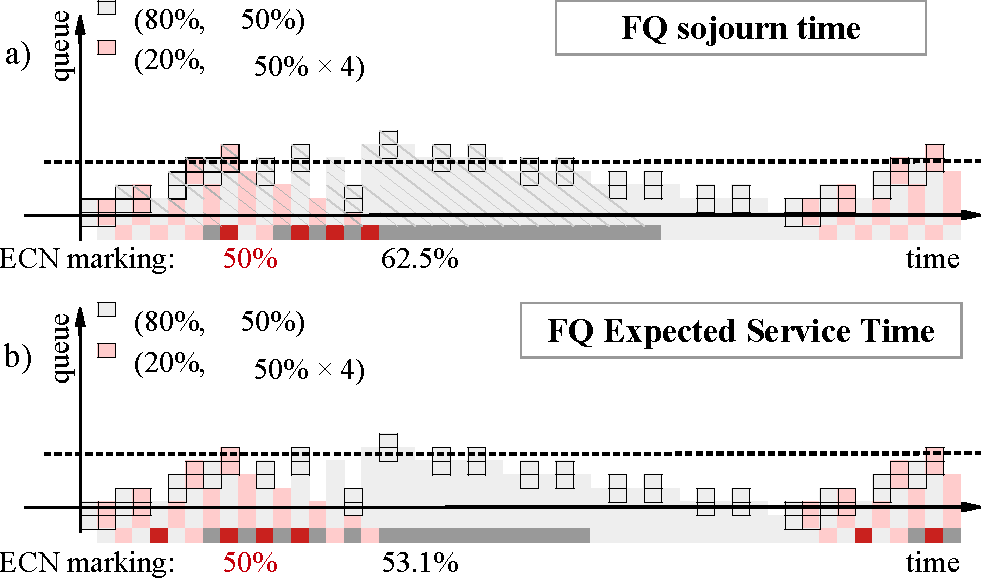
\includegraphics[width=\columnwidth]{fq-marking-fairness8020_4}
	\caption{FQ's (lack of) isolation of the grey flow from the pink is unchanged, even if the pink flow paces its burst at the same rate as the grey, but for a quarter of the time.}\label{fig:fq-marking-fairness8020_4}
\end{figure}

To complete the comparison, \autoref{fig:fq-marking-fairness8020_4} shows how FQ handles the case where the pink flow is paced at the same rate as the grey, but for only a quarter of the time. Still FQ does not isolate the grey flow from this much milder form of pink burstiness. Indeed, the grey queue and its marking is identical to the case where the pink burst all arrives in one timeslot. Nonetheless, pink marking is reduced to 50\%, which remains unchanged irrespective of the metric and irrespective of whether the grey flow reduces its rate.
      % Problem
% !TeX root = sigqdyn_tr.tex
% ================================================================
\section{The Time to Measure the Service Time of a Queue}\label{sec:svc_time}

In around 2012, it became recognized that one of the main problems with AQMs was the sensitivy of their configuration to changing environments. For example:
\begin{itemize}
	\item access links often change their rate when modems retrain in response to interference. 
	\item a queue can be part of a scheduling hierarchy and traffic in higher priority queues varies the capacity left for a lower priority queue, rapidly varying the drain rate that the AQM experiences.
	\item the capacity of radio links varies rapidly over time~\cite{McGregor10:Minstrel_TR}.
\end{itemize}

The CoDel algorithm~\cite{Nichols12:CoDel} proposed to solve this problem by measuring the queue in units of time, rather than bytes. This made the configuration of the thresholds in the algoithm independent of the drain rate.

Actually, as far back as 2002, 
Kwon and Fahmy~\cite{Kwon02:Load_v_Queue_AQM} had advised that the queue should 
be measured in units of time. Also, in 2003, S{\aa}gfors \emph{et al} had 
modified the Packet Discard Prevention Counter (PDPC+~\cite{Sagfors03:PDPC_vary}) 
algorithm by converting queue length to queuing delay to cope with the varying 
link rate of 3G wireless networks.

PDCP still measured the queue in bytes, but then converted the result to time by dividing by the link rate, which it measured over a brief interval. 

CoDel proposed an elegant way to measure the service time of the queue by adding a timestamp to each packet's internal metadata on enqueue. Then at dequeue, it subtracted this timestamp from the system time. It called the result the sojourn time of the packet. It was also pointed out that this sojourn time could be measured over an arbitrarily complex structure of queues, even across distributed input and output processors.

Because PIE~\cite{Pan13:PIE} was initially designed for implementation using existing hardware, it did not measure the service time of the queue directly using the time-stamping approach of CoDel.
Instead, like PDPC, it converted queue length to queuing delay using a regularly updated 
estimate of the link rate, measured over a set amount of packets. When there were insufficient packets in the queue to measure the link rate or the rate was varying rapidly, PIE's estimate of the link rate became stale. So in later specifications of PIE~\cite{Pan17:PIE}, it recommended the sojourn approach of CoDel that had been designed for software implementation.

The queue length (in bytes or an equivalent unit), also called the backlog, can be measured instantaneously when a packet is enqueued or when it is dequeued. Whereas sojourn time can only be measured once a packet is dequeued. 

It minimizes delay if the signal is applied at dequeue. However, in some hardware pipelines the process of preparing link layer frames, including potential encryption, compression and framing, is already in progress by the time a packet is dequeued. So it is too late to mark or drop a packet. This is one reason that PIE initially applied the congestion signal when it enqueued a packet. That is, it probabilistically dropped (or ECN-marked) the packet when it enqueued it. This signal then worked its way through the queue before being transmitted, adding a sojourn time of delay to the signal. This is still the case for DOCSIS PIE, but software variants of PIE now apply marking or dropping at dequeue. 

The matrix in \autoref{tab:added-delay} shows the delay added to the signal by various techniques for measuring queue delay (horizontal) and the two choices for where to apply the signal (vertical). It uses the following terminology: \(t_r\) is the duration used to sample the drain rate and \(t_s\) is the sojourn time. 
\begin{table}[h]
\begin{center}
\begin{tabular}{m{0.17\columnwidth}|*{3}{m{0.2\columnwidth}}}
			& \multicolumn{3}{c}{Technique to measure queue delay}\\
     where signal is applied  
			& Sojourn time
						& Time-based backlog
											&  Scaled sojourn time\\\hline 
	at enq  & \(2t_s\)	& \(t_r + t_s\)	& \(3t_s/2\)\\
	at deq  & \(t_s\)	& \(t_r\)			& \(t_s/2\)
\end{tabular}
\end{center}
\caption{Delay added to congestion signal by three different measurement techniques}%
\label{tab:added-delay}
\end{table}

The centre column shows the effective delay added by the simple `time-based backlog' technique proposed below. It also applies to the variant of that technique called `size-adjusted thresholds' below. The right hand column shows another technique, which can be used where the ability of sojourn time to measure delay across a complex set of queues is required. Nonetheless, for a simple queue, the time-based backlog is preferable, because it always adds minimal measurement delay, but not so little that it becomes too sensitive to measurement errors.

It can be clearly seen that applying a signal at enqueue adds \(t_s\) to the signal delay.
So signalling at enqueue would only be appropriate if it were not possible to mark (or drop) a packet at the head of the queue, e.g.\ due to implementation or timing constraints.

The time-based backlog approach is similar to PIE, but \(t_r\) can be as low as the serialization time of 2 packets (and they do not have to be queued together). In contrast, the IETF specification of PIE recommends that the drain rate needs 16 packets to get a representative estimate, so \(t_r\) will be the time from the centre of this estimate, that is the time to dequeue 8 packets. Also PIE's measurement becomes stale whenever there are less than 16 packets in the queue. 

The sojourn time approaches apply down to a lone packet, but they take longer to measure whenever the queue is longer, e.g.\ during a burst.

\section{Fairer Marking}\label{sec:fairer_marking}

This section introduces fairness problems when existing AQM approaches mark flows with different degrees of burstiness. Then it uses a worked example to give better intuition for how to make marking fairer. The question of what marking is actually fair is deferred to a later discussion section (\S\,\ref{sec:marking_fairness_discuss}). Here the discussion is confined to removing obvious fairness problems, which is why the title is not `Fair Marking'.

When the Random Early Detection (RED) AQM algorithm was first proposed fairness was one evaluation factor~\cite[\S\,8]{Floyd93:RED}, where fairness in the context of marking was defined as ``the fraction of marked packets for each connection is roughly proportional to that connection’s share of the bandwidth''\footnote{The paper went on to explain that ``RED gateways do not attempt to ensure that each connection receives the same fraction of the total throughput.'' Note: in the RED paper, `connection' meant a unidirectional flow.}.

Such fairness would be sufficient if all flows were long lived and smooth, but they are not.  Wischik~\cite{Wischik99:Mark_Fairly} contrives a simple two-flow scenario to demonstrate how RED can shift nearly all the marking from a burst in one flow onto a smoother flow that continues after the burst. %In this scenario one flow usually sends at a lower rate than the other, but then suddenly causes congestion by sending faster for a brief period before returning to its lower rate. The queue smoothing algorithm within the RED AQM delays nearly all the congestion marking until after the congested period ends, when most arrivals are from the constant flow. 

Classical AQMs like RED or more recent designs such as CoDel or PIE are designed to filter out variations in the queue over a likely maximum round trip. So they inherently introduce smoothing delay of about 100--200\,ms prior to signalling congestion, which is far too long to be able to mark packet bursts correctly. More recently, the importance of immediate congestion signalling has been recognized in approaches such as Data Center TCP (DCTCP~\cite{Alizadeh10:DCTCP}) and Low Latency Low Loss Scalable throughput (L4S~\cite{Briscoe16a:l4s-arch_ID}), where the job of smoothing out variations is shifted from the AQM to the sender.

Nonetheless, we will now demonstrate that even the delay spent measuring sojourn time is enough to cause immediate marking to miss packet bursts, and hit smoother flows instead. 

\begin{figure}[h]
	\centering
	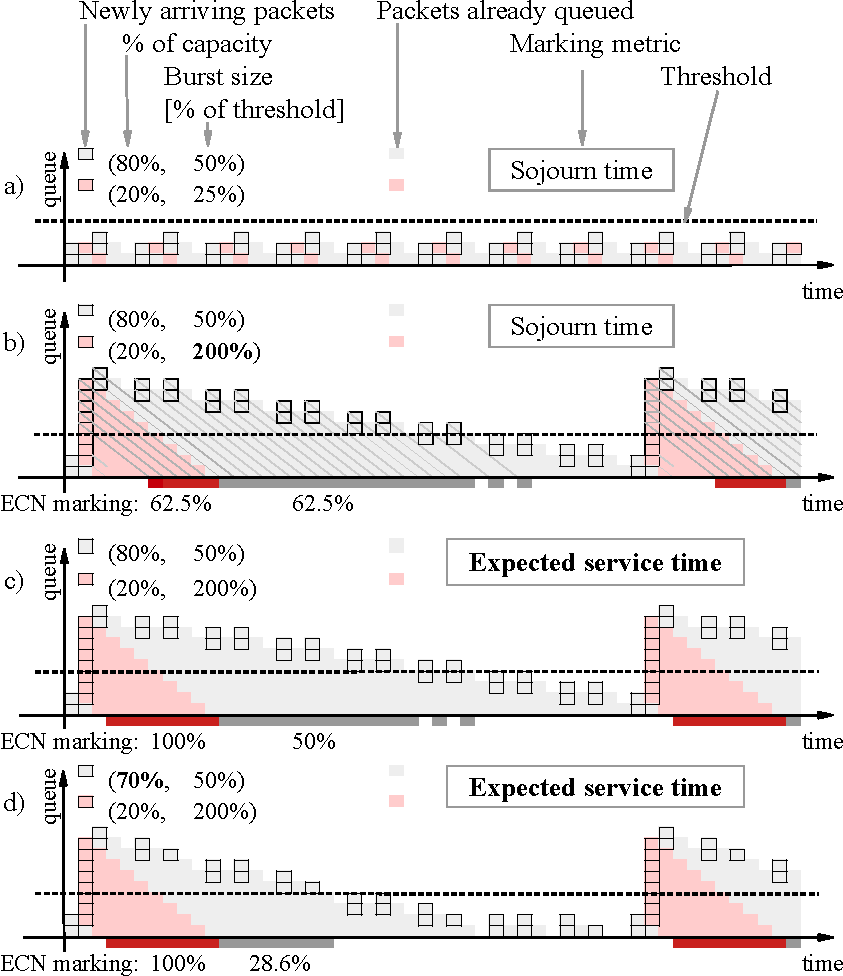
\includegraphics[width=\columnwidth]{marking-fairness}
	\caption{The Marking Fairness Problem with the Sojourn metric (b) and the ECN marking outcomes of a Solution (c--d) (see text for commentary)}\label{fig:marking-fairness}
\end{figure}

\autoref{fig:marking-fairness} shows a progression of four scenarios, reduced to their essentials by using equisized packets; one timeslot per delivered packet; a constant rate link; no congestion control; and a step ECN marking threshold. In the first three scenarios (a--c), two flows (grey and pink) fully utilize the link, consuming 80\% and 20\% each and the grey flow arrives in bursts that occupy half the queue delay threshold in the buffer. Below the progression of traffic scenarios is described, then the marking outcomes in a second pass:
\begin{enumerate}[nosep, label=\alph*)]
	\item This is the baseline case to show that the pink flow can fill the capacity left by the grey flow without exceeding the threshold, as long as it keeps its bursts small enough (in this case just 25\% of the threshold, making at most 75\% if one were to coincide with a grey burst). 
	\item In this case, each burst from the pink flow occupies 200\% of the threshold in the buffer and arrives when one packet of a grey two-packet burst is left in the queue. The average rate of both flows is unchanged, so the link is still 100\% utilized, but the grey flow still arrives in the same pattern of small bursts. So, in the time the pink burst takes to drain, some grey bursts back up behind it and, while they are draining, more small grey bursts accumulate. So the queue only finally empties just as the cycle starts to repeat.
	\item The arrivals in this scenario are identical to (b), but the marking algorithm is different (see later).
	\item In this last case, the pink flow stays unchanged at 20\% of the link and still in large bursts twice the depth of the threshold. However, the flow rate of the grey flow reduces from 80\% to 70\% of the link by halving every fourth burst. This is an attempt to represent the grey flow starting to respond to ECN marking, while the pink flow remains unresponsive.
\end{enumerate}
The ECN marking outcome of each is as follows:
\begin{enumerate}[nosep, label=\alph*)]
	\item There is no ECN marking in this baseline case (whatever the metric).
	\item The sojourn times of 5/8 of the packets at the tail of the pink burst exceed the threshold. So the sojourn-based AQM marks 62.5\% of the pink packets at dequeue. Because grey packets back up behind the pink burst, then behind themselves, their sojourn time exceeds the threshold for the first 62.5\% (5/8) of the grey packets between each pair of pink bursts. Thus, the marking probability of the two flows is equal, even though the pink flow is a lot more bursty.
	\item Here the evolution of the queue is identical to scenario (b), but marking is based on a metric we call `expected service time' rather than sojourn time. This will be fully explained in \S\,\ref{sec:exp_svc_time}, but for now it is enough to say that it marks a packet just before it is dequeued based on whether the backlog \emph{at that instant} is expected to need longer than the threshold to drain. This increases the pink marking probability from 62.5\% to 100\%. In contrast, marking shifts away from grey packets, as grey marking reduces from 62.5\% to 50\%.
	\item As the load from grey traffic falls a little, the queue falls below the threshold considerably sooner, considerably reducing the grey marking probability. Indeed a reduction of the grey traffic by 1/8 reduces grey marking probability by more than 3/8 (from 50\% to below 29\%). Nonetheless, the AQM still marks 100\% of the pink packets, because the backed up grey packets still exceed the threshold for the whole period while the pink burst is draining.
\end{enumerate}

The wider space of scenarios like this has been investigated by varying the relative shares and relative burst sizes between flows (see \S\,\ref{sec:marking_fairness_discuss}). Although the difference between the sojourn and expected service time metrics is sometimes less dramatic and sometimes more, the following intuition is generally true for all scenarios.

A smoother flow has smaller but more frequent arrival events compared to a bursty flow. So, although the bursty flow might happen to back up behind one of the smaller bursts of the smoother flow, multiple arrival events of the smoother flow will back up behind the larger burst. Therefore proportionately more of a bursty flow will be near the head of the buffer, and the packets of a smoother flow will be more likely to be occupying the tail.

Therefore, marking the head packet when there is an excessive backlog behind it is likely to lead to fairer marking than marking the head packet because it had an excessive backlog in front of it (during its sojourn through the queue). 

% ================================================================
\section{Solution: Expected Service Time}\label{sec:exp_svc_time}

Two approaches will be proposed to minimize signalling delay. Both start with the backlog measured instantaneously at dequeue, then translate it into the expected time needed to drain this backlog---thus both measure the `expected service time':
\begin{itemize}[nosep]
	\item Time-based backlog;
	\item Scaled sojourn time.
\end{itemize}

\subsection{Time-Based Backlog}\label{sec:time-based_backlog}

In this approach, as each packet is about to be dequeued from the head of the queue, the. expected service time to clear the backlog behind it is calculated as
\[\mathbb{E}(\mathrm{svc\_time}) = \mathrm{(backlog\_deq)}\times \frac{\mathrm{avg\_serializn\_time}}{\mathrm{(avg\_pkt\_size)}},\]
or in English, the expected service time, \(t_b^*\), to clear the backlog is the backlog at dequeue, \(b\) (e.g.\ in bytes), multiplied by the recent average serialization time of each packet, \(t_s^*\) and divided by the recent average packet size (in bytes), \(s^*\).

Multiplying by the quotient on the right is the same as dividing by the average drain rate. As with averaging any rate, the quotient should be calculated as a quotient of averages, not an average of quotients. This is particularly important if the drain rate varies considerably. Also the averages should be exponentially weighted moving averages (EWMAs) with high gain, e.g. \(g=\sfrac{1}{2}\), so that they respond rapidly to changing delivery rate. The gain should be an integer power of 2 so that it can be implemented as a bit-shift.

For instance, assuming the times when dequeue of the previous packet started and ended were stored as \(t_1\) \& \(t_2\) and the packet size was \(s\), the EWMAs would be updated as
\begin{align}
	t_s^* &= g\left((t_2-t_1) - t_s^*\right)\notag\\
	s^*   &= g(s - s^*)\notag
\intertext{The expected time to clear the backlog is then,}
	t_b^* &= b * t_s^* / s^*.\label{eqn:t-based_backlog}
\end{align}
While the buffer is non-empty, the time that dequeue ends, \(t_2\) will typically become the time that serialization of the next packet starts. Reusing the same time value for both will ensure that any error introduced by coarse clock precision is averaged out. 

On the other hand, if the buffer was empty when the previous packet finished dequeuing, the time that serialization took has to be used, without including the idle time waiting for the next dequeue to start.

Note that any media acquisition delay should not be counted, and the backlog that builds while waiting to acquire the medium should not be counted for AQM marking, because it is not caused by the load from the sender, and therefore cannot be reduced by getting the sender to slow down.

\subsubsection{Rationale for Time-Based Backlog}\label{sec:time-based_backlog_justify}

The time-based backlog approach assumes that the drain rate to clear the backlog will be similar to that averaged over the last few packets. There is no reason to believe that the recent drain rate is the best estimate of the rate at which the backlog will drain. For instance, a radio link is continually testing different rates to find which is the best and if a queue is continually yielding to a higher priority queue, it will proceed in fits and starts. However, for the purpose of signalling congestion, the recent drain rate gives the best available estimate of the time to drain the backlog, which itself was a result of the recent drain rate.

It should be pointed out that sojourn time also measures the drain rate over the last few packets. But it is indisputable that it is better to use a recent drain rate to estimate how fast the current backlog will drain, rather than just measuring how long it took an earlier backlog to drain that happened to be in front of the head packet when it arrived---while ignoring the current backlog.

One might consider estimating the recent drain rate from the size of just the single most recent head packet and the time to dequeue it. However, such an approach is prone to errors due to coarse clock precision or interruptions affecting access to the clock. By using EWMAs, any such errors should average out, while using a high gain keeps the measurement lag down to about two packets.

The time-based backlog approach is similar to that used in PIE, except with PIE the backlog is divided by the average drain rate over sixteen contiguous packets, and whenever the queue is not that long, the last available average rate is used.

\subsubsection{Size-Adjusted Threshold(s)}\label{sec:time-adj_thresh}

The following technique is really just an optimization of the time-based backlog. It avoids the per-packet division in \autoref{eqn:t-based_backlog} above.

It is easiest to explain with an example AQM algorithm. Say, for instance that the AQM marks packets if queuing delay exceeds a simple step threshold, \(T\). Then, as each packet is dequeued, instead of comparing the time-based backlog with the threshold queuing delay, the AQM marks a packet if
\begin{equation}
	b * t_s^* \ge s^* * T.
\end{equation}
In other words, instead of using the average packet size to scale down the backlog, it is used to scale up the threshold.

A similar approach would be used for other AQM functions. For instance, if the likelihood of marking increases by a linear ramp function, both the min and max thresholds of the ramp would be scaled up by \(s^*\).

An alternative optimization would be to ammortize the per packet calculation over a certain number of packets by accumulating the combined dequeue times of a certain number of packets and accumulating the sum of their sizes. Then every so often updating the two EWMAs, and calculating \(s^* * T / t_s^*\) to give a new threshold in bytes to compare the backlog against. However, the per-packet processing cost of the original size-adjustment is already fairly minimal (two adds, a bit-shift and two integer-multiplies).

\subsection{Scaled Sojourn Time}\label{sec:scaled_svc_time}

Another approach would be to scale the sojourn time by the ratio of the backlogs at dequeue and enqueue. That is, the expected service time at any instant would be:
\[\mathbb{E}(\mathrm{svc\_time}) = \mathrm{sojourn\_time} \times \frac{\mathrm{backlog\_deq}}{\mathrm{backlog\_enq}},\]
where \(\mathrm{backlog\_enq}\) can be written into the packet's metadata at enqueue, along with the arrival time, which is how sojourn time is already implemented.

\subsubsection{Rationale for Scaling Sojourn Time}\label{sec:inst_svc_time_justify}

Scaled sojourn time is comparable to the above `time-based backlog' approach, but with the drain rate measured over the sojourn time of each head packet, which is equivalent to \(\mathrm{backlog\_enq}/\mathrm{sojourn\_time}\). There are two disadvantages, but one advantage, to measuring over a sojourn time.
\begin{description}
	\item[Disadvantage 1:] The measurement delay depends on the queuing delay, which makes it problematic to signal bursts quickly;
	\item[Disadvantage 2:] Each sojourn measurement is sensitive to errors reading the clock and, when the ratio of the backlogs is large, as it is during a burst, any error will be greatly magnified;
	\item[Advantage 1:] Like sojourn time, scaled sojourn time can be measured over an arbitrarily complex set of queues, by only measuring the time of first enqueue and last dequeue and the backlog at enqueue and dequeue times.
\end{description}

Scaled sojourn time would not normally be of interest because of the two disadvantages. However, where an existing deployment or a complex queue structure makes the other approaches infeasible, the advantage of scaled sojourn time might outweigh these disadvantages (but see \S\,\ref{sec:sojourn-distrib}).

Scaling the sojourn time might also make more sense if an implementation is already measuring the sojourn time for another reason. Then it will not need any additional measurement code, because it might already need to maintain the backlogs to do basic queue handling.

\begin{figure}[h]
	\centering
	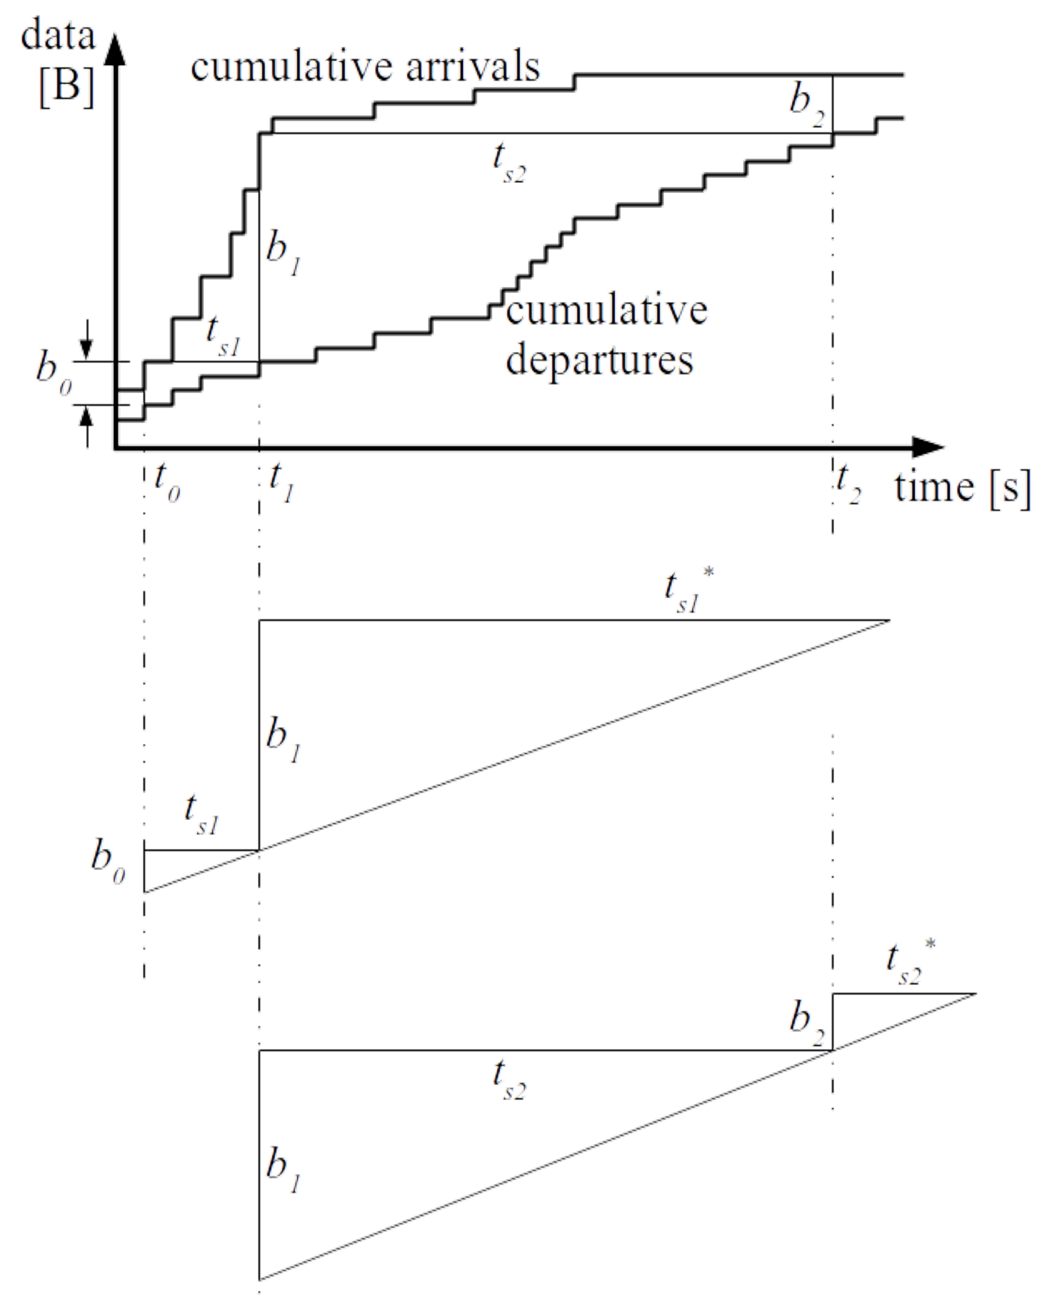
\includegraphics[width=\columnwidth]{scaled-sojourn}
	\caption{Rationale for Scaling Sojourn Time}\label{fig:scaled-sojourn}
\end{figure}

\autoref{fig:scaled-sojourn} visualizes a geometric interpretation of the rationale for scaling the sojourn time. The two plots in the chart at the top of the figure show cumulative arrivals and departures of data in packets. Between times \(t_0\) and \(t_1\) a burst of packets arrives and between \(t_1\) and \(t_2\) a few packets arrive at first, then none. Over the whole time the departure rate is varying independently as, for example, a radio link would. At any time, for instance \(t_1\), the sojourn time  (\(t_{s1}\)) can be visualized as the horizontal distance back from the departures plot to the arrivals plot. And the backlog is shown as the vertical distance between the plots (\(b_1\)).

It can be seen that the sojourn time (\(t_{s1}\)) between \(t_0\) and \(t_1\) takes account of the departure rate, but not the arrival rate (the burst), during that time. It is proposed to scale the sojourn time by the ratio of the backlogs at departure and arrival of the packet. That is \(t_{s1}^* = t_{s1} b_1/b_0\). This scaled sojourn time uses all the latest information available at time \(t_1\). 

The schematic in the middle of the figure shows, using similar triangles, how scaled sojourn time is constructed.  The departure rate during the sojourn is represented by the slope of the smaller of the middle triangle. The larger triangle extrapolates that departure rate to predict the time (\(t_{s1}^*\)) that it will take for the most recent backlog to drain.

The lower schematic shows the situation at time \(t_2\). The actual sojourn time of the new head packet \(t_{s2}\) is slightly shorter than the prediction \(t_{s1}^*\). From this new actual sojourn time, a new prediction can now be constructed  from the slightly steeper rate slope. This time the backlog \(b_2\) has reduced  during the sojourn of the head packet, because there has been a lull in arrivals since \(t_1\). Therefore the formula predicts that the sojourn time will be scaled down relative to its measured value.

We will now return to time \(t_1\) and derive the scaled sojourn time algebraically, rather than geometrically. The departure rate during the sojourn of the head packet is
\begin{align}
	r_{d1} &= \frac{b_0}{t_{s1}}.\label{eqn:drate}
\intertext{The expected service time to drain the backlog at \(t_1\) is}
	t_{s1}^* &= \frac{b_1}{r_{d1}}.\notag
\intertext{Substituting from \autoref{eqn:drate}:}
				&= t_{s1} \frac{b_1}{b_0}.\label{eqn:sojourn}
\end{align}

The expected service time can also be expressed in terms of a ratio of average arrival and departure rates during the sojourn, \(r_{a1}\) and \(r_{d1}\). The backlog at \(t_1\) can be expressed in terms of the arrival rate over the sojourn time:
\begin{align}
	b_1 &= t_{s1} r_{a1}.\label{eqn:backlog}
\intertext{Substituting this into \autoref{eqn:sojourn}, the scaled sojourn time at \(t_1\),}
	t_{s1}^* &= t_{s1} \frac{r_{a1}}{r_{d1}}
\end{align}
That is, scaling the sojourn time by the ratio between the backlogs at dequeue and enqueue is equivalent to scaling it by the ratio between the average arrival and departure rates between enqueue and dequeue.

\subsubsection{Implementing Scaled Sojourn Time}\label{sec:inst_svc_time_impl}

To implement scaling of the sojourn time, it is probably easiest to store \texttt{backlog\_enq} in the packet's metadata when the packet is enqueued. Then at dequeue it can be divided into \texttt{backlog\_deq}. 

But some implementations choose not to do too much at dequeue, because there is limited time between the packet reaching the head of the queue and starting to be forwarded. Therefore, it could be challenging to measure the system time, subtract the stored timestamp then also scale the result by a ratio.

The division in the ratio can be avoided by in at least two ways:
\begin{itemize}[nosep]
	\item Multiply the threshold(s) of the AQM by \texttt{backlog\_enq} rather than dividing it into \texttt{backlog\_deq} (as in \S\,\ref{sec:time-adj_thresh});
	\item Use the techniques below to optimize execution, although efficiency will be machine-architecture-dependent, and precision is only to the nearest binary order of magnitude:
\end{itemize}

{\small\texttt{qdelay <<= (lg(backlog\_deq) - lg(backlog\_enq)\\+ 1/2)}}\\
It is roughly equivalent to multiplying by the ratio between the backlogs, to the nearest integer power of 2.

The \texttt{<<=} operator bit-shifts \texttt{qdelay} to the left by the expression on the right. \texttt{lg()} is the logarithm function base 2. The expression bit-shifts \texttt{qdelay} to the left by the difference between the logs of the backlogs at enqueue and dequeue. The addition of 1/2 is necessary so that integer truncation of the result will round to the nearest integer, rather than always rounding down. 

The \texttt{clz()} function to count leading zeros could be used as a cheaper but more approximate base-2 log function, as follows:\\
{\small\texttt{qdelay <<= (clz(backlog\_enq) - clz(backlog\_deq))}}\\
This also avoids the need for any boundary checking code.

For example, if the \texttt{backlog\_*} variables are 32-bit unsigned integers and
\begin{itemize}[nosep]
	\item[] \texttt{backlog\_enq = 3000}, so \texttt{clz(3000)=20}
	\item[] \texttt{backlog\_deq = 30000}, so \texttt{clz(30000)=17}
\end{itemize}
Then
\begin{itemize}[nosep]
	\item[] \texttt{qdelay <<= 20 - 17}
\end{itemize}
is the same as
\begin{itemize}[nosep]
    \item[] \texttt{qdelay *= 2\^{}3},\\
\end{itemize}
which scales qdelay by 8, which approximates to \texttt{30,000/3,000 = 10} but is an integer power of 2. This is sufficient to scale the sojourn time to the correct binary order of magnitude, while still taking account of all the latest information in the queue.

However, \texttt{clz()} introduces truncation bias because it always rounds down, which could lead the result to be persistently out by up to \(\times2\) or \(/2\) for a particular target sojourn time. Using the \texttt{lg()}-based expression could be out by from \(\sqrt{2}\) to \(1/\sqrt{2}\), but with no bias---it is equally likely to be out either way.

A high performance implementation will maintain the backlog of a queue by maintaining two variables (much like the two plots at the top of \autoref{fig:scaled-sojourn}):
\begin{itemize}[nosep]
	\item[] \texttt{count\_enq} written solely by the enqueue routine;
	\item[] \texttt{count\_deq} written solely by the dequeue routine
\end{itemize}	
Then the backlog can be measured as \texttt{count\_enq - count\_deq}. These two shared variables can be read from any routine, but they are only incremented by the routine that owns them, which avoids the performance hit of a mutual exclusion lock. The two counters monotonically increase like the system clock for the sojourn measurement, but at the rate of data transfer in and out respectively, not the rate of time passing. 

\subsection{Distributed Queues}\label{sec:sojourn-distrib}

Using sojourn time leverages the advantage that it can be measured across a complex set of queues, including the case where the initial enqueue and the final dequeue routines are distributed across different machines or processors, as already mentioned (separate clocks would need to be synchronized).

This could include the case where the inputs are located on multiple client machines (e.g.\ mobile user equipment, WiFi stations, cable modems or passive optical network modems) while the output is a located at an aggregation node (e.g.\ a cellular base station (eNodeB)~\cite{Tan09:AQM_uplink_patent}, a WiFi access point (AP), a centralized controller for multiple WiFi APs, a cable modem terminal server (CMTS) or optical line termination (OLT) equipment), with a multiplexed access network between the clients and the aggregation node.

In complex cases like these, if minimization of measurement delay is important, the best approach to use will depend on which of metrics are most feasible to measure and communicate to the dequeue process, which will depend on the architecture of the distributed queues. \autoref{tab:distrib-qs} tabulates which metrics are needed by which approach.

\begin{table*}[h]
	\begin{center}
		\begin{tabular}{ll|cc}
						& 				& Time-based backlog & Scaled sojourn time\\
			\hline
			\multirow{2}{*}%
			{enqueue time}& arrival time		& -					& \checkmark \\
						& backlog				& -					& \checkmark \\
			\hline
			\multirow{4}{*}%
			{dequeue time}& departure time		& \checkmark		& \checkmark \\
						& backlog				& \checkmark		& \checkmark \\
						& serialization time	& \checkmark		& - \\
						& packet size			& \checkmark		& - \\
		\end{tabular}
	\end{center}
	\caption{Metrics needed by each approach}%
	\label{tab:distrib-qs}
\end{table*}

Note that the backlog at enqueue time and the backlog at dequeue time need to include all the data buffered between the two, not just that in the ingress and egress buffers. Therefore the backlog metric is probably the critical factor for feasibility. And given both approaches need the backlog at dequeue time, and scaled sojourn also needs the backlog at enqueue time, scaled sojourn might end up being the more complex approach.`

For instance, on a single machine, the \texttt{count\_enq} variable would be available in a memory shared between ingress and egress. But if the ingress and egress are separate, the ingress machine would have to communicate the \texttt{count\_enq} variable to the egress over a (preferably non-blocking) control channel, so that the egress could calculate \texttt{backlog\_deq} by subtracting \texttt{count\_deq}. 

Certain access network technologies, e.g.\ those for cellular radio access networks, already include such a control channel, over which buffer status report (BSR) control messages are sent from the user equipment at the ingress to the radio network controller. The delay to access a control variable at the input machine from the output machine would be larger than that in a non-distributed system, but it would at least be a known, constant delay. So the control system could still provide robust metrics to control queuing in the data channel.

As well as the aggregation node using expected service time (EST) to apply congestion signalling within the final dequeue routine (effectively on behalf of the input queue), the aggregation node could also use EST to govern the scheduling algorithm for controlling each client's inward (upstream) access rate into the shared medium, by altering the rate at which it granted medium access slots to each client.

\subsection{Applicability of Expected Service Time}\label{sec:inst_svc_time_applic}

Using any of the approaches in \S\,\ref{sec:exp_svc_time} to calculate EST would improve timeliness relative to using sojourn time or other techniques to measure queue delay. However, it would not be worth modifying an existing deployment unless all other delays were going to be removed at the same time. 

It might be thought that an algorithm like the proportional integral (PI) controller\footnote{Used in QCN~\cite{IEEE802.1Qau:Ethernet_QCN}, PIE~\cite{Pan17:PIE}, PI2~\cite{DeSchepper16a:PI2} or the base AQM of DualPI2~\cite{Briscoe15e:DualQ-Coupled-AQM_ID}.} already takes account of the change in queuing delay between samples, so changing the queuing delay measurement itself seems redundant. However, using EST actually ensures that a PI algorithm takes account of the change between the latest queue delay measurements at each sample time, not between two outdated measurements.

It might also be thought that PI controllers do not need to care so much about instantaneous measurements, because they are maintaining the fairly large queue that is needed by classic TCP algorithms like Reno, Cubic, Compound or BBR. However, even though a PI algorithm only samples the queue fairly infrequently (relative to packet serialization time), using an out of date queue metric makes it necessary to introduce extra heuristic code to deal with the resulting sloppiness.

For instance, in the case of PIE~\cite{Pan17:PIE}, some heuristic code suppresses any drop once the last sample of queue delay falls below half the target delay.\footnote{As long as some other conditions hold that are not important here.} This is an attempt to suppress drop when the queue is draining after the load has gone idle. However, it is ineffective if sojourn time is used to measure the queue, because the sojourn time does not reduce until after the last packet (as explained on the right of \autoref{sojourn-prob}). Using EST whenever it is sampled should eliminate the need for this heuristic because it takes account of the reducing backlog as the queue drains.\footnote{Indeed, this was the original motivation for this work.}

EST is also applicable to the CoDel algorithm for the same reasons---sojourn time fails to take account of the evolution of the queue after the head packet was enqueued (again, as in \autoref{sojourn-prob}). This can tend to cause the AQM to continue dropping or marking packets at the end of a flow, because the sojourn time does not recognize that the queue has gone below the target delay. The CoDel code in Linux includes a heuristic to exit dropping mode when the backlog goes below 1\,MTU, but that still continues dropping mode until the last packets of a flow, and tail loss is particularly problematic for a flow to detect.

EST is particularly applicable to a simple AQM algorithm like the time-based shallow threshold recommended for DCTCP in~\cite{Bai16:MQ-ECN} or the native AQM for L4S traffic in DualPI2~\cite[Appx.\ A]{Briscoe15e:DualQ-Coupled-AQM_ID} or Low Latency DOCSIS~\cite{CableLabs:DOCSIS3.1}. It would be applicable whether the threshold is a simple step, or a probabilistic ramp like the RED function (but based on instantaneous queue delay, not smoothed queue length), or a deterministic ramp or convex function of instantaneous queueing delay, as in Curvy RED~\cite[Appx.\ B]{Briscoe15e:DualQ-Coupled-AQM_ID}. The queue in these cases is intended to be very shallow, so it might seem that the extra measurement delay would be minimal. However, the sensitivity of these very low delay schemes to burstiness makes it particularly important to ensure that bursts are measured rapidly and correctly.

EST could apply to many types of queue, not just packet queues, as long as the size of each job is quantified in common units that are additive. Examples include, but are not limited to, queues of datagrams, frames or packets, as well as message queues, call-server queues, computer process scheduling queues, storage queues (e.g. SSD or disk), workflow queues for mechanical or human-operated stages of tasks. 

As well as dropping or ECN-marking, different sanctions could be applied using the same basic ideas. Examples include, but are not limited to: truncating or otherwise damaging the data or checksum of a message or packet but preserving the information necessary for delivery; rerouting; delaying; downgrading the class of service; and tagging.

% ================================================================
\section{Marking Fairness}\label{sec:marking_fairness_discuss}

\subsection{Marking Fairness Experiments}\label{sec:marking_fairness_expts}

\todo{ToDo: Experiments with sojourn-based marking to compare against EST-based below}

\begin{figure*}[t!]
	\centering
	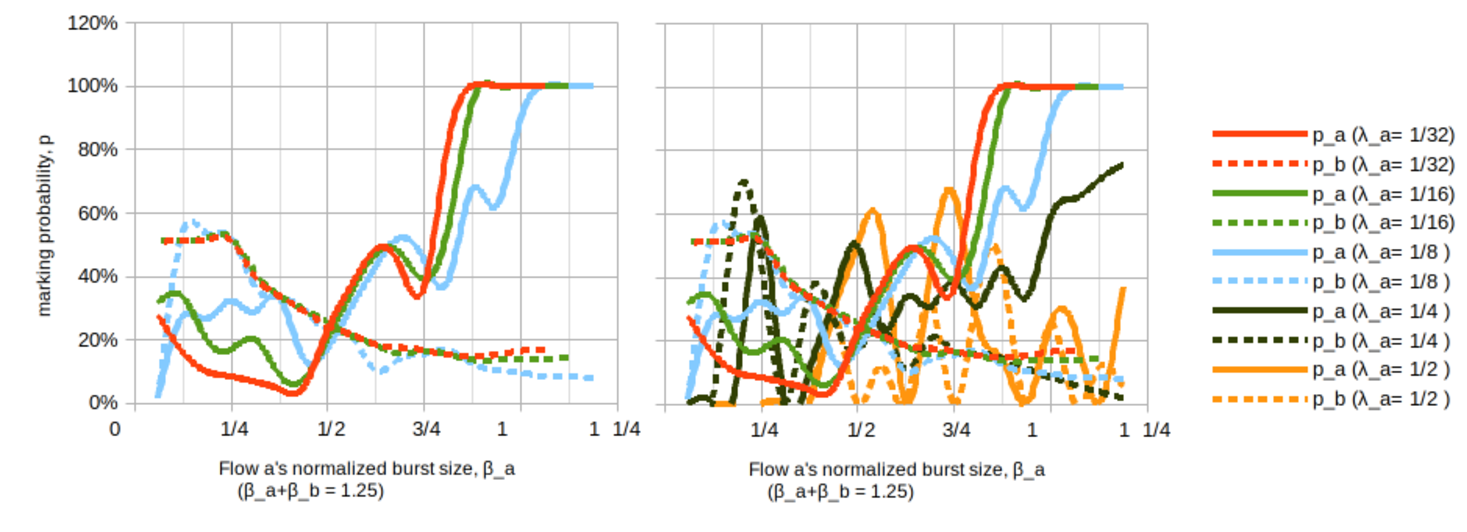
\includegraphics[width=\linewidth]{marking-fairnessSumBeta125}
	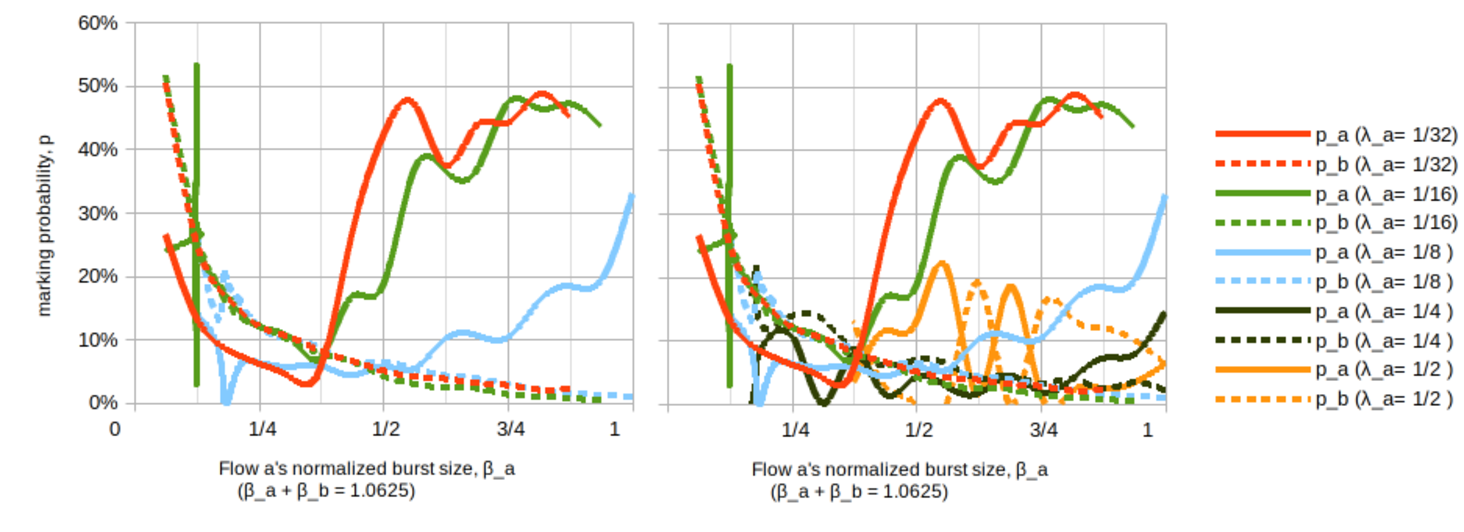
\includegraphics[width=\linewidth]{marking-fairnessSumBeta10625}
	\caption{Marking fairness of two flows wrt capacity share, \(\lambda\), and relative burstiness, \(\beta\).\\
	\(\lambda_a+\lambda_b=100\%; \quad\mathrm{top:} \beta_a+\beta_b=1.25; \quad\mathrm{bottom:} \beta_a+\beta_b=1.0625\). 
	The left-hand charts are the same as the right, except they exclude two scenarios that otherwise obscure the other plots}\label{fig:marking-fairness-range}
\end{figure*}

\autoref{fig:marking-fairness-range} shows the degree to which ECN marking is or is not focused onto the more bursty of a pair of flows indexed as \(a\) \& \(b\). Both flows were modelled as unresponsive and two timeslots were used for the smaller burst in a similar way to the example in \autoref{fig:marking-fairness}b). So the results are not necessarily an accurate reflection of a real AQM, but they should at least be indicative of the likely outcome.

The charts show the ECN marking level that results from scanning the scenario parameters across two dimensions:
\begin{enumerate}
	\item The capacity share of flow \(a\), \(\lambda_a\) is varied from \sfrac{1}{32} to \sfrac{1}{2} and the share the other flow \(b\) is also varied so that it fills the remainder of the link (\(\lambda_a+\lambda_b=100\%\))). The left-hand chart of each pair is identical to the right-hand chart except, to help pick out the plots, the last two capacity-share scenarios are omitted.
	\item The normalized burst size of flow \(a\), \(\beta_a\) is increased from \sfrac{1}{16} in steps of \sfrac{1}{16}, while the burst size of flow \(b\) is reduced such that the sum of both burst sizes is constant. The sum is 1.25 in the top plots, and 1.0625 in the bottom. 	Normalization is relative to the ECN marking threshold, so a sum of 1.25 means that if bursts from both flows coincide, a previously empty queue would exceed the marking threshold by 25\%.
\end{enumerate}

It can be seen from the right-hand side of any of the plots that, if flow \(a\) utilizes a small fraction of the capacity (up to roughly \sfrac{1}{8}) and if it is even slightly more bursty than the flow \(b\) (which is using more of the capacity), EST-based marking focuses a high fraction of the marking onto the more bursty flow. Still focusing on the right hand-halves (where flow \(a\) is more bursty than \(b\)), stepping down the scenarios as flow \(a\) uses more of the capacity, it still attracts more of the marking than \(b\) but the bias against it reduces. By the time \(a\) is using half the capacity, it's marking is still generally higher than \(b\) but the difference continually narrows, even where \(a\) is considerably more bursty than \(b\).

It is also noticeable that wobbles increasingly appear; some so great that at certain points, even when sharing capacity 50:50, the more bursty flow attracts \emph{less} of the marking. \todo{It is possible that these wobbles are an artefact of the model, so a more precise simulation will be necessary.}

By comparing the top charts with the bottom in \autoref{fig:marking-fairness-range}, it can also be seen that, a higher combined level of burstiness pushes the marking level of the more bursty flow up to 100\% over a wider range of capacity shares. This trend continues as combined burstiness increases further than shown. For instance when flow \(a\) bursts to 2\(\times\) the threshold, and \(b\) bursts to \(\sfrac{1}{16}\), \(a\) attracts 100\% marking for any capacity share up to 50\%.

\subsection{What Marking would be Fair?}\label{sec:marking_fairness_definition}

As remarked in \S\,\ref{sec:fairer_marking} it is obvious when marking is extremely unfair. For instance, if a bursty flow is using fraction \(\lambda\) of the capacity on average, but attracting less than fraction \(\lambda\) of the marking. However, it is not obvious how much more marking it would be fair to apply to a flow for bursts of a particular size relative to those of another flow.

The doctoral research of Wischik~\cite{Wischik99:Mark_Fairly, Wischik99:Large_Dev_PhD} and sample path shadow pricing~\cite{Kelly98:Shadow_prices_prop_fair} on which it is based appear to be the only work to tackle the question of how to define fair marking. Wischik considers a number of possible definitions of fair marking, which is reduced down to the following three candidates, all of which are intended for offline analysis only, not for a live marking algorithm. Also all are defined in relation to packet loss, and all assume high statistical multiplexing of flows at a resource:
\begin{description}
	\item[Effective bandwidth:] EB was developed in the context of flow admission control. The EB of a variable rate flow is somewhere between its mean and peak throughputs. A bursty flow can replaced by another flow with the same effective bandwidth without altering the resulting loss probability, including replacement by a flow with constant throughput equal to the effective bandwidth. So it would be fair to mark flows in proportion to their effective bandwidths.
	\item[\boldmath\(\Delta{L}\):] The function \(L(Y)\) is defined as the volume of loss at a resource when presented with load \(Y\). Then \(\Delta{L(Y)}\) is the change in the loss volume when the flow under consideration is removed, which is the standard definition of a shadow price, so should provide the basis for fair marking. 
	\item[Sample Path Shadow Pricing:] SPSP (\autoref{fig:spsp}) marks every packet that, if removed, would have resulted in one less packet being dropped.
\end{description}

\begin{figure}[h]
	\centering
	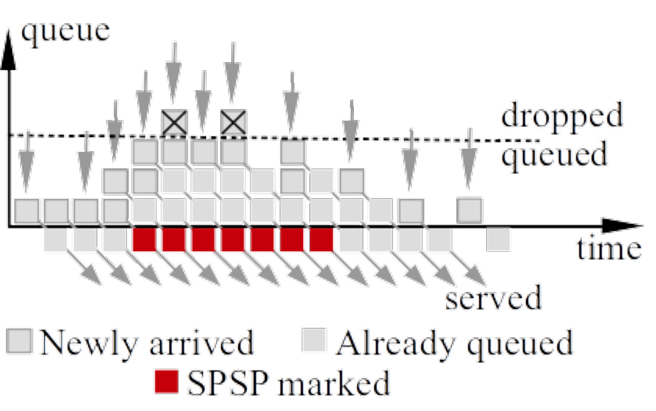
\includegraphics[width=0.8\columnwidth]{spsp}
	\caption{Schematic of Sample Path Shadow Pricing (SPSP) with one timeslot per equisized packet for illustration. A packet is marked (in red) if removing it would have resulted in one less packet being dropped}\label{fig:spsp}
\end{figure}

Wischik explains that each definition has aspects in common with the others, but they differ in their goals, assumptions and user models. 

\(\Delta{L}\) suffers from not being `incrementally fair'. As flows are added to the load, even if they are equally bursty and of equal average throughput, the rise in the volume of loss is greater for each additional flow added. So, with a certain load, imagine that the \(\Delta{L}\) due to removing any one flow is 0.3\%, but removing two equal flows reduces loss by only 0.5\%. Then if two flows band together, and internally share the marks they get under the \(\Delta{L}\) scheme between themselves, they would get only 0.25\% marking each, thereby proving that \(\Delta{L}\) is not incrementally fair.

In contrast, SPSP is incrementally fair because it acts at the granularity of packets, and is agnostic to whether packets band together under flows or users. This also means that SPSP is concerned with precisely which packets to mark, whereas \(\Delta{L}\) only knows what proportion of marks to allocate to each flow.

Like \(\Delta{L}\), EB can only say what proportion of marks should be applied to each flow but EB only knows the relative proportions; it does not know how many marks to apply overall, although this can be remedied if an exchange rate between drops and marks is defined. 

Thus, in the words of Wischik, ``SPSP is best''. However, like all the schemes, SPSP can only be applied offline---in retrospect. In the case of SPSP, this is because it is meant to mark the packets that were in the queue as it built up to the point of overflow, but many of those packets will already have left the queue by the time the queue does overflow (for instance the first four marked packets in \autoref{fig:spsp}).

Nonetheless, SPSP represents an ideal scheme that a practical marking algorithm
ought to aspire to. %Wischik proposes a marking algorithm that does just that.
% It is called Reach Overload, Send ECN (ROSE) and works as follows. Whenever
% the queue size exceeds a threshold, mark all packets in the queue. The
% threshold, \(b\), is adaptively determined as follows: for every packet that
% would have been marked by SPSP, decrease \(b\) by \(\kappa\epsilon\). For
% every packet that is marked, increase \(b\) by \(\epsilon\) \(\epsilon\) is a
% small fixed quantity and \(\kappa\) represents the number of marks that are
% equivalent to a drop, which Wischik recommends should be somewhat greater than
% one for robustness.
However, the goals of the present work are wider than those in Wischik. We particularly want to maintain very low queuing delay, but we do also want to ensure marking is as fair as possible. Therefore, it will be worth taking note of the two questions that Wischik poses to assess the fairness of a marking algorithm:
\begin{enumerate}[nosep]
	\item Does it marks packets that caused overflow, or does it mark innocent packets that arrived later?
	\item Does it mark in the busy period leading up to the overflow?
\end{enumerate}
\begin{figure}[h]
	\centering
	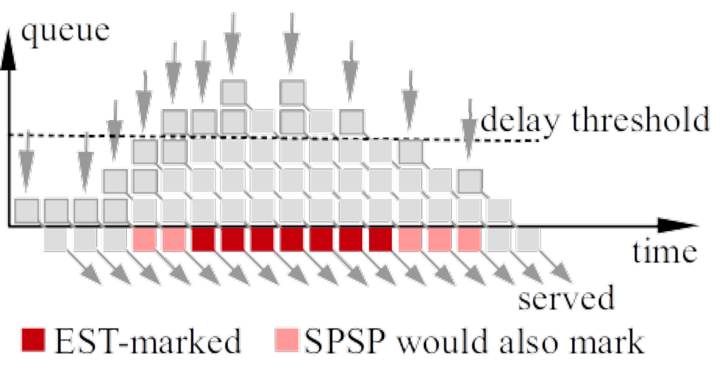
\includegraphics[width=0.9\columnwidth]{est-spsp}
	\caption{Marking based on Expected Service Time compared against Sample Path Shadow Pricing}\label{fig:est-spsp}
\end{figure}
For marking based on expected service time (EST), we redefine overflow as exceeding the queuing delay target (in time units not bytes). Then, using the example scenario in \autoref{fig:est-spsp}, we can answer the questions and justify where EST diverges. 

\begin{enumerate}[nosep, label=Q\arabic*.]
	\item EST does not mark any innocent packets; however it does not mark the packets that contributed to excess delay but were dequeued after excess delay had ended (the pink packets to the right of the red ECN-marked packets). 
	\item EST marks as many packets in the busy period leading up to excess delay as possible, but it cannot mark those that had already been served when excess delay was first detected (the pink packets to the left).
\end{enumerate}
From the earlier analysis of EST-based marking of traffic bursts, it can be seen that EST will rarely miss any packets in the build-up to excess delay, because most of the packets of a burst are still queued when the tail arrives. Also stopping EST marking as soon as the excess delay has gone away seems preferable for two reasons:
\begin{itemize}
	\item It seems less likely to hit smoother flows, which tend to back up behind a burst, as explained in \S\,\ref{sec:fairer_marking};
	\item When there has been a period of marking, the load arriving from sources will reduce a round trip later. Thus if marking were to continue until the queue was empty, it would tend to cause under-utilization in the following round trip.
\end{itemize}

\subsection{Queue Protection and Marking Fairness}\label{sec:qprot_marking_fairness}

\todo{Subsection to discuss potential for Queue Protection without per-flow state and ACK Asad for the initial idea.}

% ================================================================
\section{Other Signalling Delays}\label{sec:other_delays}

The introduction enumerated six causes of delay to congestion signals and highlighted two that this memo would focus on. The other four sources of signalling delay are briefly surveyed below, with pointers to where they have been considered in other work.

\subsection{Propagation Delay} Numerous proposals have been made to speed up signalling by sending the signal from the queue back against the flow of traffic, direct to the sender. This can be done in a pure L2 network, e.g. backwards congestion notification (BCN) in IEEE 802.1Qau~\cite{IEEE802.1Qau:Ethernet_QCN} a.k.a.\ Quantized Congestion Notification (QCN), which is now rolled into 802.1Q-2011 and 802.1Q-2014. However, in general signalling backwards is problematic in IP networks, amongst other reasons because the sender has to accept out-of-band packets from any arbitrary source in the middle of the network, which makes it vulnerable to DoS attacks~\cite{IETF_RFC6633:ICMP_SQ_Depr}. 

Therefore, here we will assume that signals are piggy-backed on the forward traffic flow then fed back to the sender via the receiver. However, this does not preclude a solution to the problems of backwards congestion notification.

\subsection{Smoothing Delay} AQMs designed for the Internet's classic congestion controls (TCP Reno, Cubic, Compound, etc.) filter out fluctuations in the queue by smoothing it before using the smoothed measurement as a measure of load to drive the congestion signal. DCTCP~\cite{Alizadeh10:DCTCP} proposed to smooth the signal at the sender, so that the network could send out the signal immediately, without smoothing, and L4S followed this approach~\cite{Briscoe16a:l4s-arch_ID}. This allows the sender to receive the signal without smoothing delay, which is particularly useful in cases where the sender might not need to smooth the signal itself, e.g.\ to detect overshoot when accelerating to start a new flow. Shifting the smoothing function from the network to the sender also makes sense because the network does not know the round trip time (RTT) of each flow, so it has to smooth over the maximum likely RTT. Whereas a sender knows its own RTT and can smooth over this timescale.

\subsection{Signal encoding delay} Previous research has proposed to change the IP wire protocol to provide more bits to signal congestion. Nonetheless, it has been pointed out\footnote{Matt Mathis is believed to have pointed this out first.} that the delay of a unary encoding is inversely proportional to the value being encoded, and the congestion window of a scalable congestion control is also inversely proportional to the value of the congestion signal. So, as flow rates (and consequently congestion windows) increase over the years, at least in general the delay to encode the signal does not increase.\footnote{However, encoding delay does increase with the degree of ACK coalescing.}

Therefore, in this report we have assumed the unary encoding of congestion signals standardized as ECN by the IETF~\cite{IETF_RFC3168:ECN_IP_TCP}. This does not preclude other encodings, e.g. the multi-bit encoding of QCN or minor alterations to the decoding to avoid saturation, such as that in \cite{Briscoe17a:CC_Tensions_TR}.

\subsection{Removing Randomness Delays}\label{sec:rand_delay}

One of the main motivations for the design of Random Early Detection (RED)~\cite{Floyd93:RED} was to break up synchronization between the sawteeth of TCP flows driving the same queue. This still remains an important requirement for all AQM algorithms~\cite{Baker15:AQM_Recommendations}.

AQMs mitigate synchronization by introducing marking or dropping more gradually than a tail-drop buffer would, and to a certain extent by randomizing the marking. 

With clean-slate approaches such as DCTCP in private networks, or incrementally deployable clean-slate approaches like L4S~\cite{Briscoe16a:l4s-arch_ID} for the public Internet, requirements for the network and for end-systems are still in the process of definition. In these clean-slate or slightly dirty-slate cases, it would be possible to require the sender's congestion control to dither its response to congestion signals, so that it would not be necessary to introduce randomness in the network, which adds uncertainty and therefore delay to the congestion signalling channel. 

Any AQM that probabilistically signals congestion with probability \(p\) could deterministically signal congestion by introducing an interval of \(1/p\) packets between each drop or mark. PDPC+~\cite{Sagfors03:PDPC_vary} and CoDel~\cite{Nichols12:CoDel}, which is very similar, use a deterministic rather the probabilistic algorithm to encode the congestion signal. Both AQMs in DualPI2~\cite[Appx.\ A]{Briscoe15e:DualQ-Coupled-AQM_ID} also uses a deterministic algorithm.

The determinism would be lost wherever the AQM was controlling flows multiplexed within one queue without per-flow state, because assignment of each deterministic congestion signal to each flow would become randomized by even slightly random packet arrivals from the different flows~\cite{Briscoe15d:PIE_rvw}.

Nonetheless, whenever a flow is on its own in an AQM, which is a common case for the traffic patterns in many access network designs,  deterministic congestion signalling would reduce signalling delay. This could particularly ease the design of new flow-start algorithms, where the flow introduces microbursts or chirps to sense at what level it starts to congest the link.

Determinism of an AQM is of less importance when the congestion control rather than the AQM determines the spacing between marks. For instance, the duration of the sawteeth of a classical congestion control scales with BDP. So at low BDP, the AQM determines the spacing between marks, but as BDP scales, the congestion control sawteeth move in and out of closed loop control, which determines the duration between `congestion events' with the AQM inactive between times~\cite[\S\,3.3]{Briscoe21c:pi2param}.      % Body
%\input{sigqdyn_tr_relwk-data}     % Related work
% !TeX root = sigqdyn_tr.tex
% ================================================================
\section{Related Work}\label{sec:related}

Scaling sojourn time seems superficially similar to combined enqueue and dequeue ECN marking (CEDM)~\cite{Shan17:CEDM}, because CEDM marks a packet at enqueue if the queue is over a threshold, but then unmarks it at dequeue if the backlog has dropped below the threshold. However the two are significantly different. Firstly, CEDM has to be based on queue length in order to mark at enqueue. But also CEDM is intentionally asymmetric, in that it unmarks packets if the backlog at dequeue has dropped below the threshold, but it does not mark packets at dequeue if they have risen above the threshold. In contrast, scaling sojourn time is deliberately symmetric, meaning it compensates for growth or shrinkage of the backlog (\autoref{fig:scaled-sojourn}).

\section{Further Work}

These ideas might not be novel, but no concerted effort has been made to search the literature. The ideas have not been evaluated either.

\section{Acknowledgements}\label{sigqdyntr_acks}

%The breakdown of the elements of signalling delay in the Introduction is based on unpublished work for the author's PhD from 2006--07 entitled ``Necessary Changes Towards a Sufficient Internetwork Protocol;
%Simple, Scalable, Secure \& Responsive Resource Control''. 
The scaling of the service time of the queue was based on discussions with Henrik Steen, an MSc student of the author, in Nov 2016 \& May 2017.      % Tail pieces (discussion, conclusions, plans, acks)
% ----------------------------------------------------------------

%\onecolumn%
%\clearpage
\addcontentsline{toc}{section}{References}

{\footnotesize%
\bibliography{aqm-details}}

% ----------------------------------------------------------------
\clearpage
%\twocolumn%
\appendix
% !TeX root = sigqdyn_tr.tex
% ================================================================
\section{Scaled Sojourn Time: Details}\label{sec:scaled_sojourn_details}

% ----------------------------------------------------------------
\subsection{Scaled Sojourn Time: Analysis}\label{sec:scaled_sojourn_analysis}

\begin{figure}[h]
	\centering
	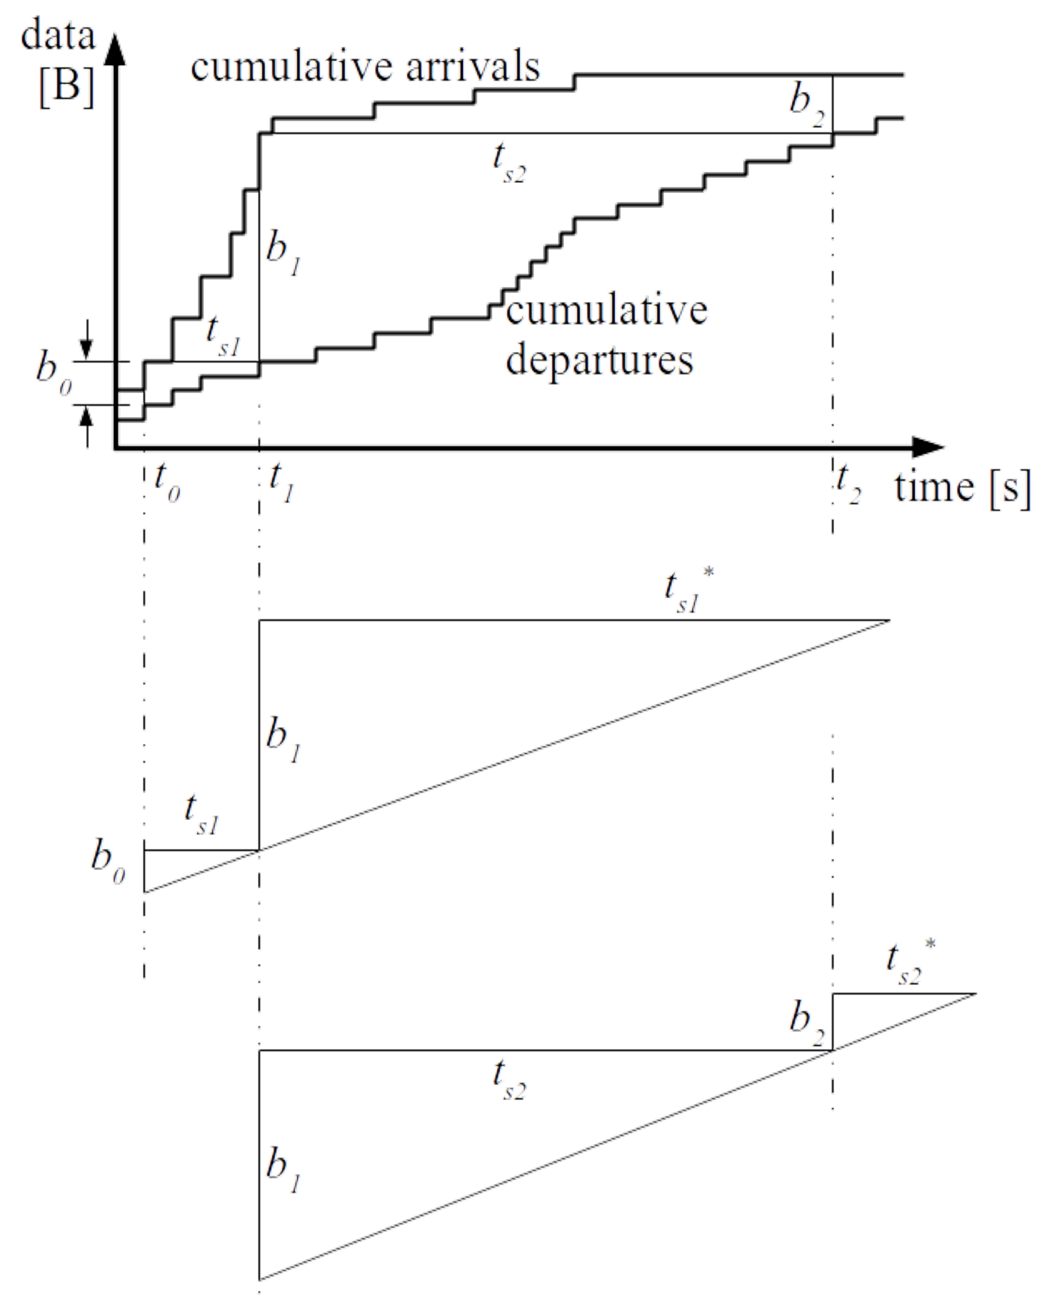
\includegraphics[width=\columnwidth]{scaled-sojourn}
	\caption{Rationale for Scaling Sojourn Time}\label{fig:scaled-sojourn}
\end{figure}

\autoref{fig:scaled-sojourn} visualizes a geometric interpretation of the rationale for scaling the sojourn time. The two plots in the chart at the top of the figure show cumulative arrivals and departures of data in packets. Between times \(t_0\) and \(t_1\) a burst of packets arrives and between \(t_1\) and \(t_2\) a few packets arrive at first, then none. Over the whole time the departure rate is varying independently as, for example, a radio link would. At any time, for instance \(t_1\), the sojourn time  (\(t_{s1}\)) can be visualized as the horizontal distance back from the departures plot to the arrivals plot. And the backlog is shown as the vertical distance between the plots (\(b_1\)).

It can be seen that the sojourn time (\(t_{s1}\)) between \(t_0\) and \(t_1\) takes account of the departure rate, but not the arrival rate (the burst), during that time. It is proposed to scale the sojourn time by the ratio of the backlogs at departure and arrival of the packet. That is \(t_{s1}^* = t_{s1} b_1/b_0\). This scaled sojourn time uses all the latest information available at time \(t_1\). 

The schematic in the middle of the figure shows, using similar triangles, how scaled sojourn time is constructed.  The departure rate during the sojourn is represented by the slope of the smaller of the middle triangle. The larger triangle extrapolates that departure rate to predict the time (\(t_{s1}^*\)) that it will take for the most recent backlog to drain.

The lower schematic shows the situation at time \(t_2\). The actual sojourn time of the new head packet \(t_{s2}\) is slightly shorter than the prediction \(t_{s1}^*\). From this new actual sojourn time, a new prediction can now be constructed  from the slightly steeper rate slope. This time the backlog \(b_2\) has reduced  during the sojourn of the head packet, because there has been a lull in arrivals since \(t_1\). Therefore the formula predicts that the sojourn time will be scaled down relative to its measured value.

We will now return to time \(t_1\) and derive the scaled sojourn time algebraically, rather than geometrically. The departure rate during the sojourn of the head packet is
\begin{align}
	r_{d1} &= \frac{b_0}{t_{s1}}.\label{eqn:drate}
\intertext{The expected service time to drain the backlog at \(t_1\) is}
	t_{s1}^* &= \frac{b_1}{r_{d1}}.\notag
\intertext{Substituting from \autoref{eqn:drate}:}
				&= t_{s1} \frac{b_1}{b_0}.\label{eqn:sojourn}
\end{align}

The expected service time can also be expressed in terms of a ratio of average arrival and departure rates during the sojourn, \(r_{a1}\) and \(r_{d1}\). The backlog at \(t_1\) can be expressed in terms of the arrival rate over the sojourn time:
\begin{align}
	b_1 &= t_{s1} r_{a1}.\label{eqn:backlog}
\intertext{Substituting this into \autoref{eqn:sojourn}, the scaled sojourn time at \(t_1\),}
	t_{s1}^* &= t_{s1} \frac{r_{a1}}{r_{d1}}
\end{align}
That is, scaling the sojourn time by the ratio between the backlogs at dequeue and enqueue is equivalent to scaling it by the ratio between the average arrival and departure rates between enqueue and dequeue.

% ----------------------------------------------------------------
\subsection{Implementing Scaled Sojourn Time}\label{sec:inst_svc_time_impl}

To implement scaling of the sojourn time, it is probably easiest to store \texttt{backlog\_enq} in the packet's metadata when the packet is enqueued. Then at dequeue it can be divided into \texttt{backlog\_deq}. 

But some implementations choose not to do too much at dequeue, because there is limited time between the packet reaching the head of the queue and starting to be forwarded. Therefore, it could be challenging to measure the system time, subtract the stored timestamp then also scale the result by a ratio.

The division in the ratio can be avoided by in at least two ways:
\begin{itemize}[nosep]
	\item Multiply the threshold(s) of the AQM by \texttt{backlog\_enq} rather than dividing it into \texttt{backlog\_deq} (as in \S\,\ref{sec:time-adj_thresh});
	\item Use the techniques below to optimize execution, although efficiency will be machine-architecture-dependent, and precision is only to the nearest binary order of magnitude:
\end{itemize}

{\small\texttt{qdelay <<= (lg(backlog\_deq) - lg(backlog\_enq)\\+ 1/2)}}\\
It is roughly equivalent to multiplying by the ratio between the backlogs, to the nearest integer power of 2.

The \texttt{<<=} operator bit-shifts \texttt{qdelay} to the left by the expression on the right. \texttt{lg()} is the logarithm function base 2. The expression bit-shifts \texttt{qdelay} to the left by the difference between the logs of the backlogs at enqueue and dequeue. The addition of 1/2 is necessary so that integer truncation of the result will round to the nearest integer, rather than always rounding down. 

The \texttt{clz()} function to count leading zeros could be used as a cheaper but more approximate base-2 log function, as follows:\\
{\small\texttt{qdelay <<= (clz(backlog\_enq) - clz(backlog\_deq))}}\\
This also avoids the need for any boundary checking code.

For example, if the \texttt{backlog\_*} variables are 32-bit unsigned integers and
\begin{itemize}[nosep]
	\item[] \texttt{backlog\_enq = 3000}, so \texttt{clz(3000)=20}
	\item[] \texttt{backlog\_deq = 30000}, so \texttt{clz(30000)=17}
\end{itemize}
Then
\begin{itemize}[nosep]
	\item[] \texttt{qdelay <<= 20 - 17}
\end{itemize}
is the same as
\begin{itemize}[nosep]
    \item[] \texttt{qdelay *= 2\^{}3},\\
\end{itemize}
which scales qdelay by 8, which approximates to \texttt{30,000/3,000 = 10} but is an integer power of 2. This is sufficient to scale the sojourn time to the correct binary order of magnitude, while still taking account of all the latest information in the queue.

However, \texttt{clz()} introduces truncation bias because it always rounds down, which could lead the result to be persistently out by up to \(\times2\) or \(/2\) for a particular target sojourn time. Using the \texttt{lg()}-based expression could be out by from \(\sqrt{2}\) to \(1/\sqrt{2}\), but with no bias---it is equally likely to be out either way.

A high performance implementation will maintain the backlog of a queue by maintaining two variables (much like the two plots at the top of \autoref{fig:scaled-sojourn}):
\begin{itemize}[nosep]
	\item[] \texttt{count\_enq} written solely by the enqueue routine;
	\item[] \texttt{count\_deq} written solely by the dequeue routine
\end{itemize}	
Then the backlog can be measured as \texttt{count\_enq - count\_deq}. These two shared variables can be read from any routine, but they are only incremented by the routine that owns them, which avoids the performance hit of a mutual exclusion lock. The two counters monotonically increase like the system clock for the sojourn measurement, but at the rate of data transfer in and out respectively, not the rate of time passing. 

      % Scale Sojourn Time: Details
% !TeX root = sigqdyn_tr.tex
% ================================================================
\section{Marking Fairness}\label{sec:marking_fairness_discuss}

\subsection{Marking Fairness Experiments}\label{sec:marking_fairness_expts}

\subsubsection{EST-based Marking Fairness}\label{sec:marking_fairness_expts_est}

\begin{figure*}[t!]
	\centering
	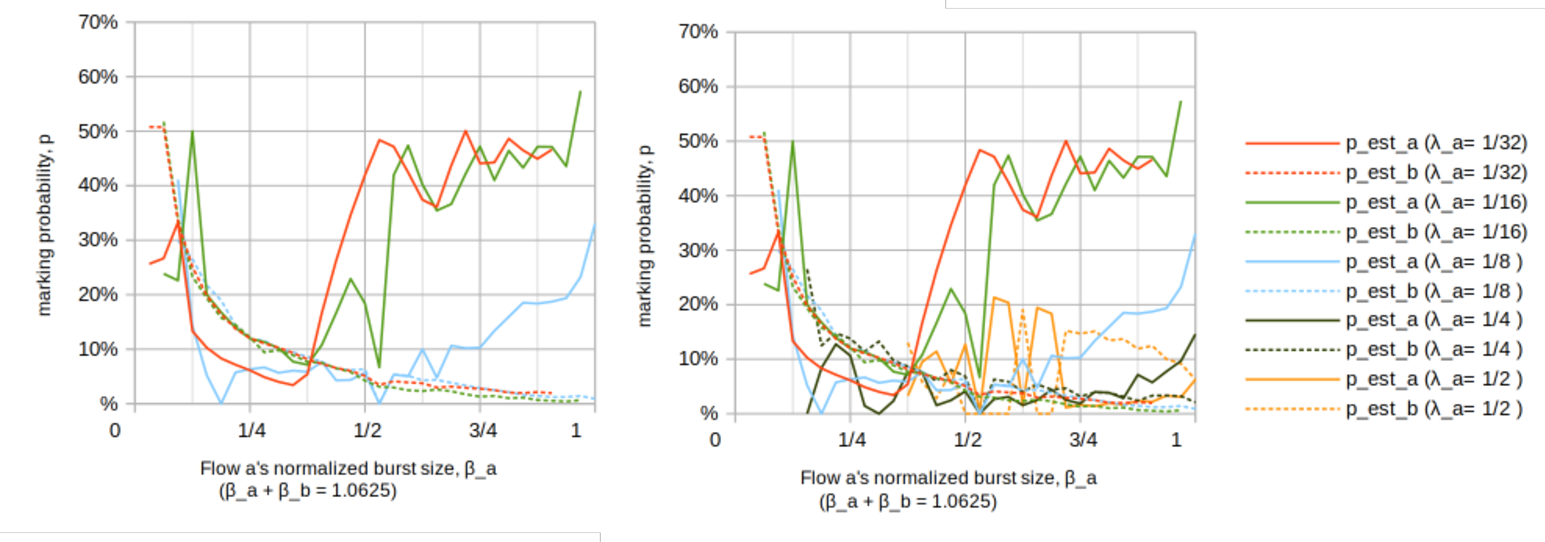
\includegraphics[width=\linewidth]{est-fairnessSumBeta10625}
	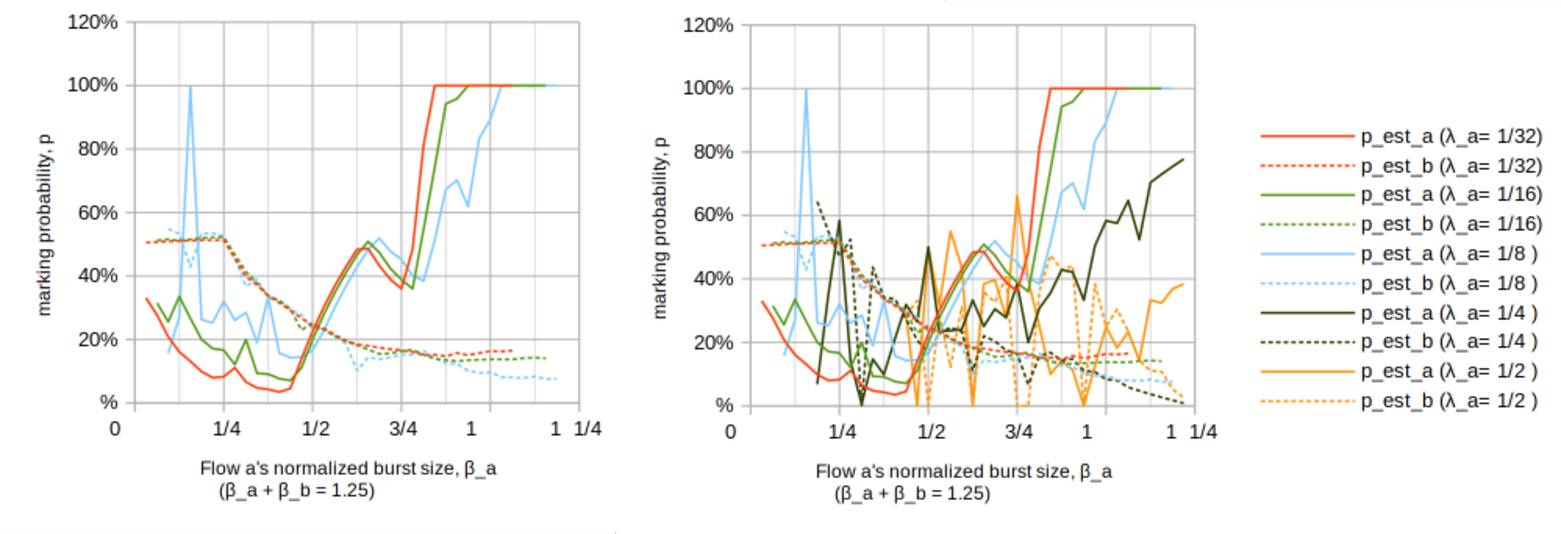
\includegraphics[width=\linewidth]{est-fairnessSumBeta125}
	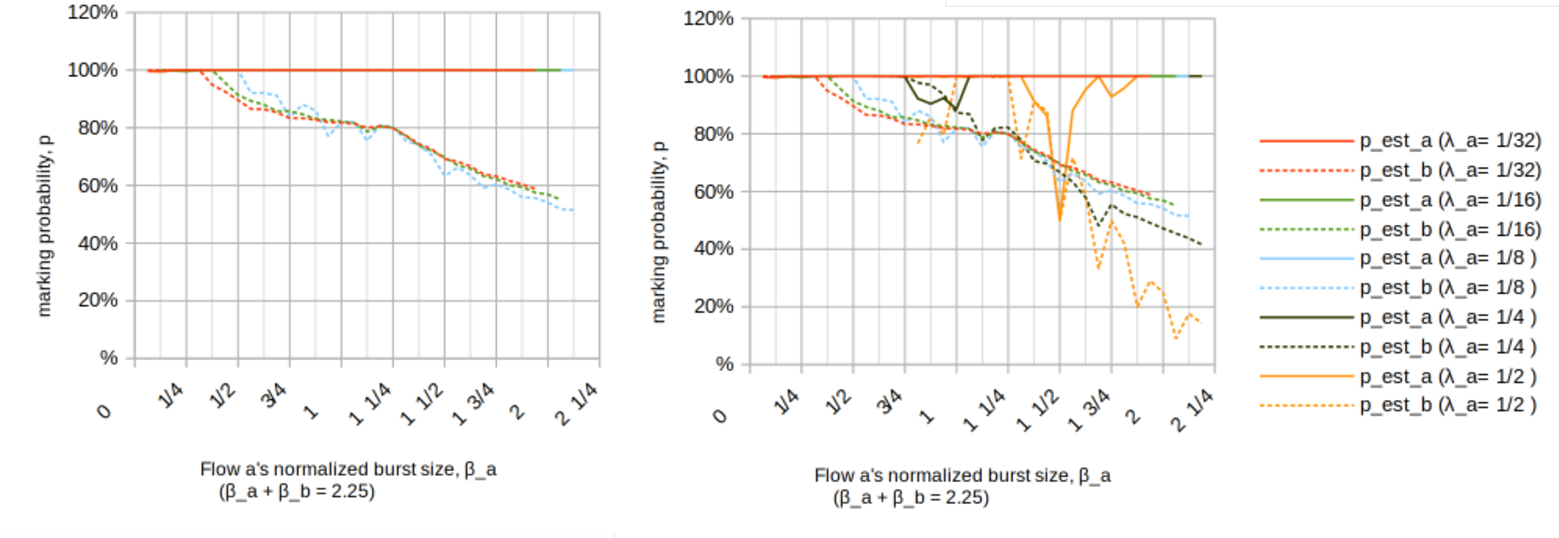
\includegraphics[width=\linewidth]{est-fairnessSumBeta225}
	\caption{EST-based marking fairness of two flows wrt capacity share, \(\lambda\), and relative burstiness, \(\beta\).\\
	\(\lambda_a+\lambda_b=100\%; \quad\mathrm{top:} \beta_a+\beta_b=1.0625; \quad\mathrm{middle:} \beta_a+\beta_b=1.25 
	\quad\mathrm{bottom:} \beta_a+\beta_b=2.25\). 
	The left-hand charts are the same as the right, except they exclude two scenarios that otherwise obscure the other plots}\label{fig:est-fairness-range}
\end{figure*}

\autoref{fig:est-fairness-range} shows the degree to which EST-based ECN marking is or is not focused onto the more bursty of a pair of flows indexed as \(a\) \& \(b\). Both flows were modelled as unresponsive in a time-slotted model similar to the example in \autoref{fig:marking-fairness5050}b). So the results are not necessarily an accurate reflection of a real AQM, but they should at least be indicative of the likely outcome.

The charts show the ECN marking level that results from scanning the scenario parameters across two dimensions:
\begin{enumerate}
	\item The capacity share of flow \(a\), \(\lambda_a\) is varied from \sfrac{1}{32} to \sfrac{1}{2} and the share the other flow \(b\) is also varied so that it fills the remainder of the link (\(\lambda_a+\lambda_b=100\%\))). The left-hand chart of each pair is identical to the right-hand chart except, to help pick out the plots, the last two capacity-share scenarios are omitted.
	\item The normalized burst size of flow \(a\), \(\beta_a\) is increased from \sfrac{1}{16} in steps of \sfrac{1}{16}, while the burst size of flow \(b\) is reduced such that the sum of both burst sizes is constant. The sum is 1.25 in the top plots, and 1.0625 in the bottom. 	Normalization is relative to the ECN marking threshold, so a sum of 1.25 means that if bursts from both flows coincide, a previously empty queue would exceed the marking threshold by 25\%.
\end{enumerate}

It can be seen from the right-hand side of any of the plots that, if flow \(a\) utilizes a small fraction of the capacity (up to roughly \sfrac{1}{8}) and if it is even slightly more bursty than the flow \(b\) (which is using more of the capacity), EST-based marking focuses a high fraction of the marking onto the more bursty flow. 

It is also noticeable that wobbles increasingly appear; some so great that at certain points, even when sharing capacity 50:50, the more bursty flow attracts \emph{less} of the marking. It is possible that these wobbles are an artefact of the time-slotting in the model, so a more precise simulation will be necessary.

Working down from top to bottom of \autoref{fig:est-fairness-range}, it can also be seen that, as the combined level of burstiness increases, it pushes the marking level of the more bursty flow up to 100\% over a wider range of capacity shares, ultimately remaining at 100\% across any share of burstiness.

However, it must be admitted that the region where the plots of flow \(a\) and \(b\) cross (for any capacity share, \(\lambda_a\)) is always to the left of centre. The capacity share of \(a\) is never more than half, so this means that there is a range to the left of centre where \(a\)'s marking probability is higher even though both its burstiness and capacity share are lower than \(b\)'s, although this inversion corrects itself as \(b\)'s relative burstiness increases.

\begin{figure*}[t!]
	\centering
	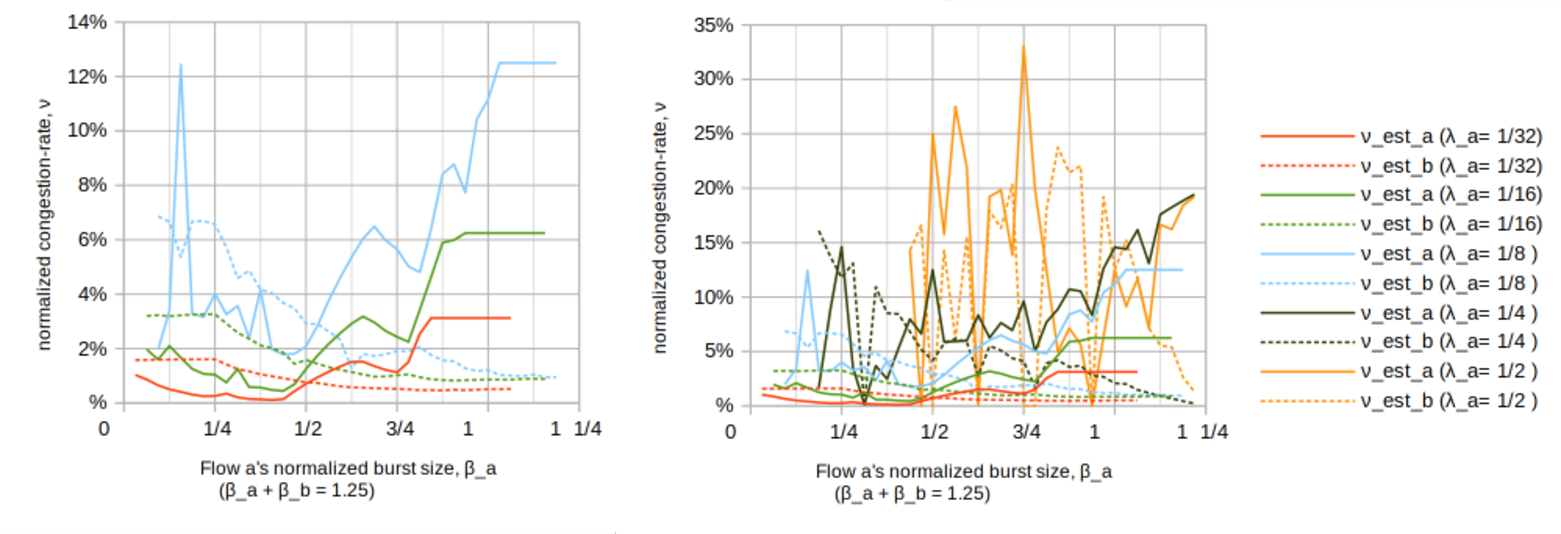
\includegraphics[width=\linewidth]{est-cong-rateSumBeta125}
	\caption{EST-based congestion-rate of two flows wrt capacity share, \(\lambda\), and relative burstiness, \(\beta\).\\
		\(\lambda_a+\lambda_b=100\%; \quad\mathrm{top:} \beta_a+\beta_b=1.0625; \quad\mathrm{middle:} \beta_a+\beta_b=1.25 
		\quad\mathrm{bottom:} \beta_a+\beta_b=2.25\) (same as \autoref{fig:est-fairness-range}). 
		The left-hand charts are the same as the right, except they exclude two scenarios that otherwise obscure the other plots}\label{fig:cong-rate-range}
\end{figure*}

Focusing again on the right hand side of the charts (where flow \(a\) is more bursty than \(b\)), it may seem counter-intuitive that those flows with a smaller share of the capacity attract a higher marking probability. Even though \(a\)'s marking probability is still generally higher than \(b\)'s, the difference continually narrows, even where \(a\) is considerably more bursty than \(b\).

The explanation is that, when the size of flow \(a\)'s bursts relative to \(b\)'s remains the same (on the same vertical), but its share of capacity increases, its bursts will become more closely spaced. Then, they are more likely to arrive behind some of \(b\)'s traffic. So flow \(a\)'s marking probability will decrease as its capacity share increases.

Also it should be kept in mind that two flows with the same burstiness (on the vertical line down the middle of the plots) would be expected to have the same marking \emph{probability} even if they have different shares of capacity. But a flow with a lesser share of the capacity will attract a proportionately lesser share of the \emph{volume} of marks. This is explained in \autoref{fig:cong-rate-range}, which shows the same traffic scenario as the middle of \autoref{fig:est-fairness-range}, but the metric on the y-axis is normalized congestion-rate, which represents the proportion of link throughput that is marked, rather than just the proportion of flow \(a\). Or formally, the normalized congestion rate of flow \(a\), \(\nu_a = \lambda_a p_a\). With this metric it can be seen that, for the same relative burstiness (same vertical), the proportion of marks increases with capacity share, as would be expected intuitively.

\begin{figure*}
	\centering
	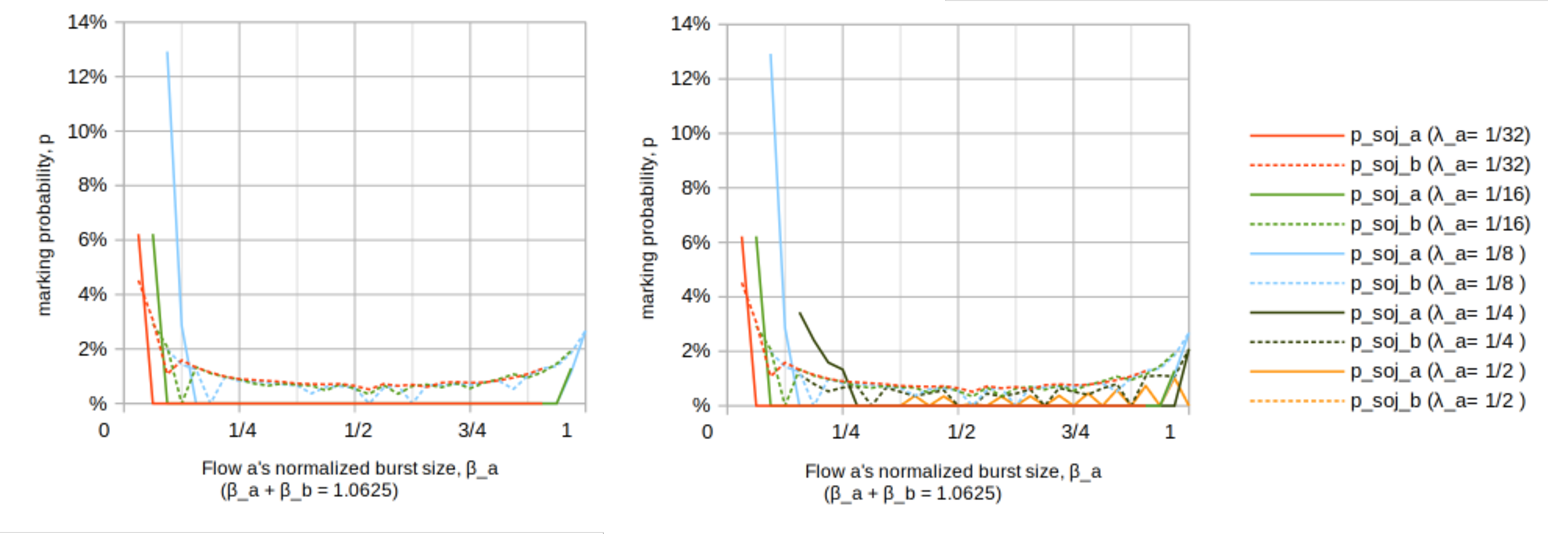
\includegraphics[width=\linewidth]{soj-fairnessSumBeta10625}
	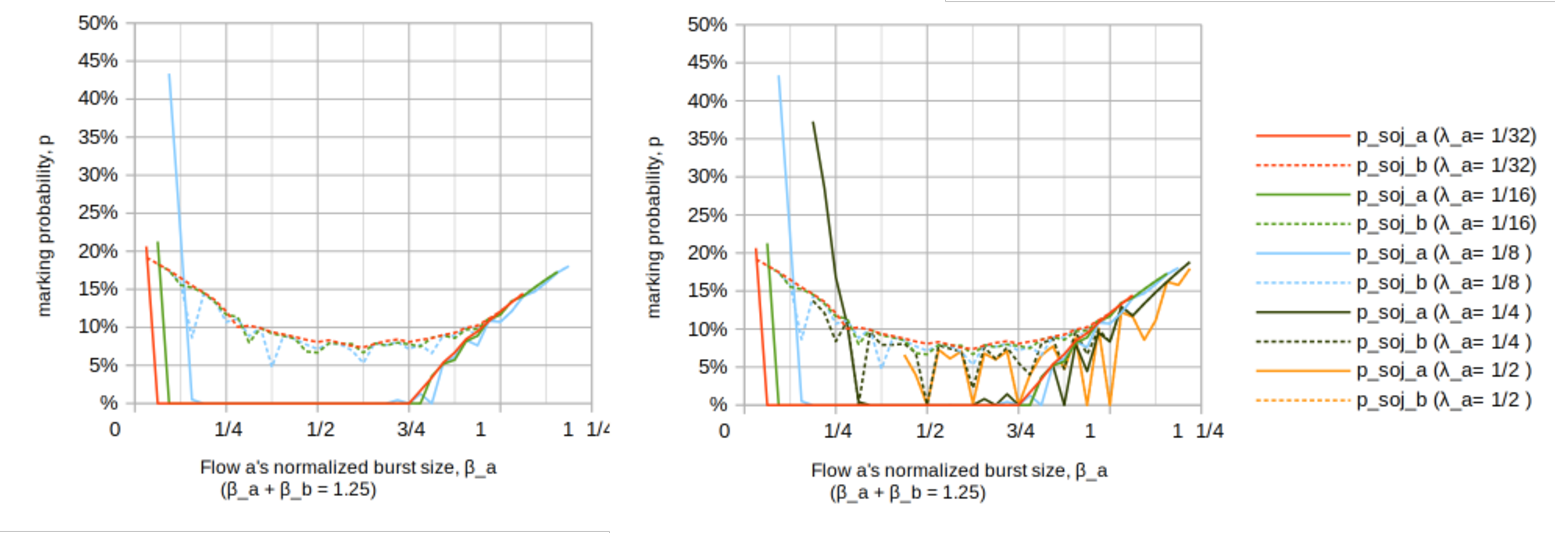
\includegraphics[width=\linewidth]{soj-fairnessSumBeta125}
	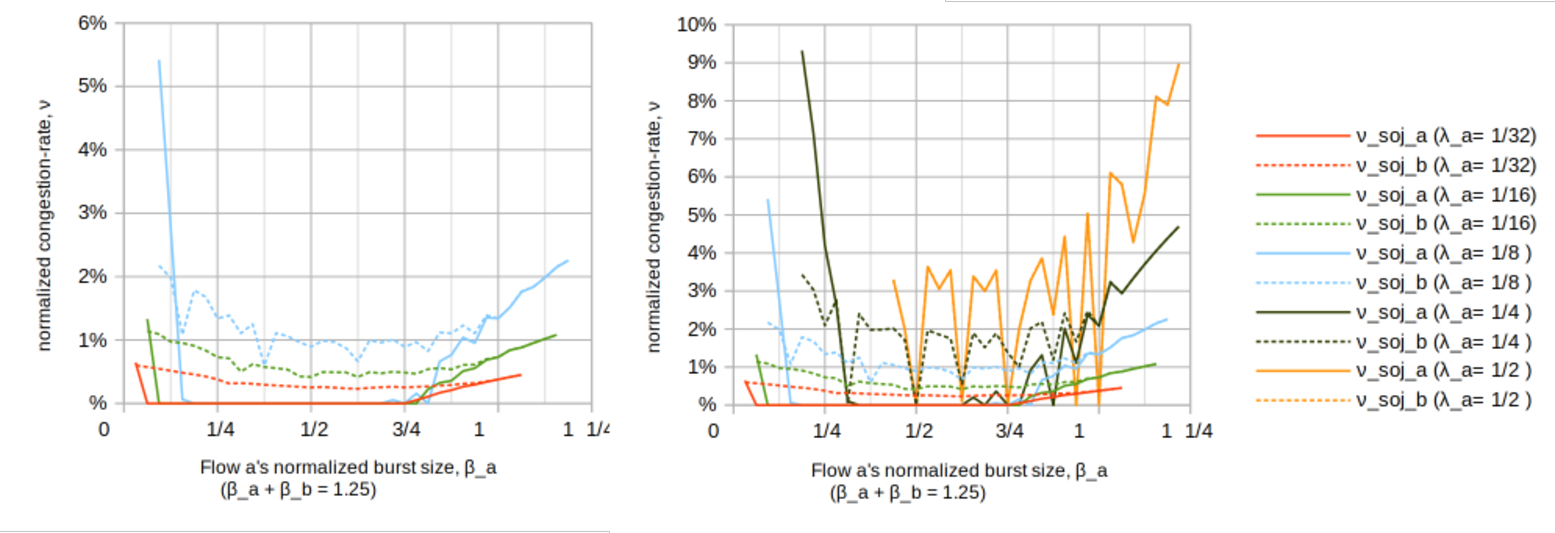
\includegraphics[width=\linewidth]{soj-cong-rateSumBeta125}
	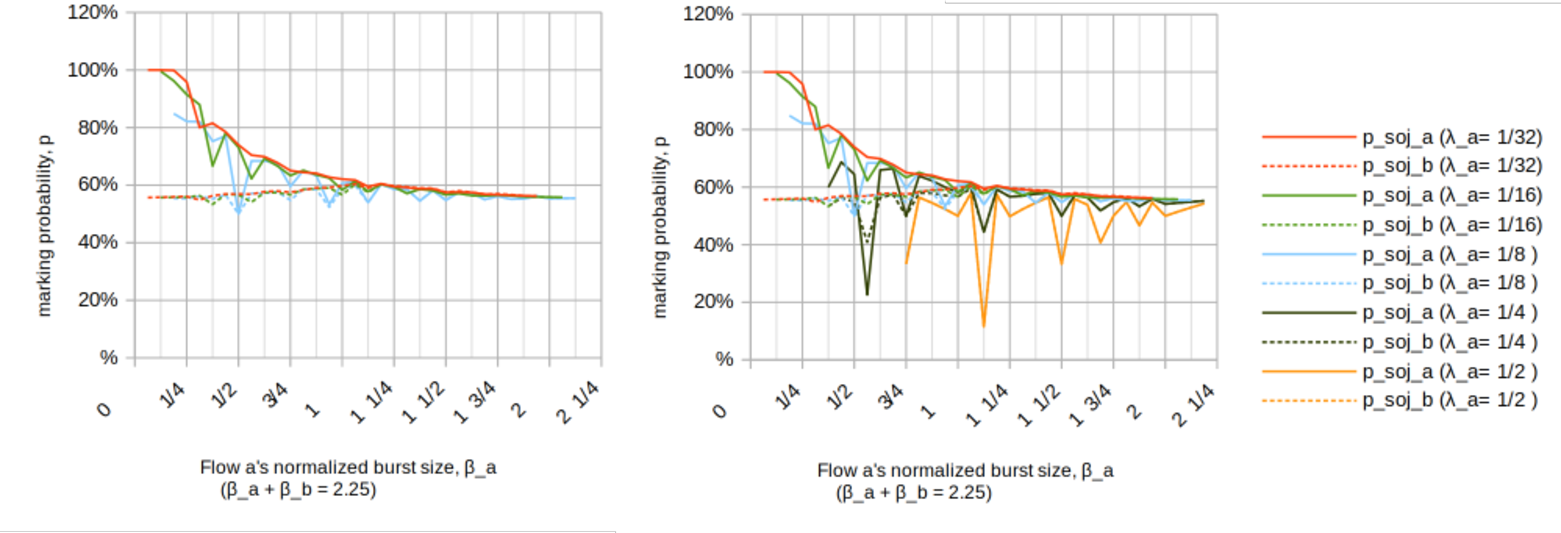
\includegraphics[width=\linewidth]{soj-fairnessSumBeta225}
	\caption{Sojourn-based marking fairness of two flows wrt capacity share, \(\lambda\), and relative burstiness, \(\beta\).\\
		\(\lambda_a+\lambda_b=100\%; \quad\mathrm{top:} \beta_a+\beta_b=1.0625;\) upper (marking prob) and lower (congestion-rate) middle: \(\beta_a+\beta_b=1.25 
		\quad\mathrm{bottom:} \beta_a+\beta_b=2.25\) (same as \autoref{fig:est-fairness-range}). 
}\label{fig:soj-fairness-range}
\end{figure*}

\subsubsection{Sojourn-based Marking Fairness}\label{sec:marking_fairness_expts_soj}

For comparison, \autoref{fig:soj-fairness-range} shows the ECN marking that results from sojourn-based marking under the same traffic scenarios as the EST-based marking in \autoref{fig:est-fairness-range} (note that the lower middle row is the same scenario as the upper middle, but the metric is normalized congestion-rate, which can be compared with \autoref{fig:cong-rate-range}).

The most obvious failing can be seen on the left-hand half of the lowest row (\(\beta_a+\beta_b=2.25\)), but also on the far-left of the other rows, where flow \(a\)'s marking exceeds \(b\)'s even though its burstiness and capacity share are both lower.
Similarly, on the right of the plots, no matter how bursty \(a\) becomes, its marking probability never exceeds \(b\)'s. Thus, sojourn-based marking sometimes perversely rewards burstiness and penalizes smoothness.

The second most obvious failing is the much lower overall marking probability in any of the scenarios, given the high degree of burstiness in all scenarios. Even when the bursts of flow \(a\) alone all exceed twice the marking threshold (\(\beta_a>2\) in the bottom row), marking is no higher than 60\% (in contrast, as  \(a\)'s bursts become smaller its marking perversely rises to 100\%). And in the middle case (\(\beta_a+\beta_b=2.25\)), even when all \(a\)'s bursts exceed the threshold (\(\beta_a>1\) the marking probability only lies in the 10\%--20\% range.

      % Marking Fairness: Comparative Evaluation
%\onecolumn%
% ----------------------------------------------------------------
%TODO

\onecolumn%
\addcontentsline{toc}{part}{Document history}
\section*{Document history}

\begin{tabular}{|c|c|c|p{3.5in}|}
 \hline
Version &Date &Author &Details of change \\
 \hline\hline
00A     & 04 Sep 2017	&Bob Briscoe &First draft.\\\hline%
01      & 05 Sep 2017	&Bob Briscoe &First complete version.\\\hline%
02      & 07 Sep 2017	&Bob Briscoe &Added a couple of refs. Qualified claims about clz().\\\hline%
03      & 16 Jan 2018	&Bob Briscoe &Completed the algebraic rationale for scaling sojourn time.\\\hline%
04		& 15 Apr 2019	&Bob Briscoe &Added abstract\\\hline%
04A		& 26 Nov 2021	&Bob Briscoe &Restructured. Generalized from Scaled Sojourn to Expected Service Time, and added Time-based Backlog as better approach. Added sections on Fairer Marking and Marking Fairness.\\\hline%
\metaversion &\metadate&Bob Briscoe &Added marking fairness results based on sojourn for comparison, and discussion and plots of congestion-rate as well as probability.\\\hline%
\hline%
\end{tabular}

\end{document}

% ----------------------------------------------------------------

%Useful section headers
%% ================================================================
%\section{}\label{sigqdyntr_}
%
%% ----------------------------------------------------------------
%\subsection{}\label{sigqdyntr_}
%
%% - - - - - - - - - - - - - - - - - - - - - - - - - - - - - - - -
%\subsubsection{}\label{sigqdyntr_}
